% DLCoEP: Recurrent Neural Networks
\section[RNN]{Recurrent Neural Networks}
% Order: the plain RNN first, then the GRU, then the LSTM, then how to read out a sequence, the case study and the summary.
\subsection{The Plain RNN}
% Colours of the presentation template, defined here as well so that the TikZ diagrams also compile in the cheat sheet.
\definecolor{nyupurple}{RGB}{90, 35, 140}
\definecolor{lightnyupurple}{RGB}{159, 120, 184}

%%%%%%%%%%%%%%%%%%%%%%%%%%%%%%%%%%%%%%%%%%%%%%%%%%%
\begin{frame}
  \begin{center}
    {\Large Recurrent Neural Network (RNN)}
  \end{center}
\end{frame}


%%%%%%%%%%%%%%%%%%%%%%%%%%%%%%%%%%%%%%%%%%%%%%%%%%%
\begin{frame}[fragile] \frametitle{Sequences}

\begin{itemize}
\item Need to predict where the ball will be at the next moment?
\item Scenario 1: no info of previous state is given. Answer: random state.
\item Scenario 2: some info of previous state is given. Answer: possible to fit trajectory and predict.
\item Another example: On mobile, while typing sms you get some predictive suggestions !!!
\end{itemize}

\begin{center}
\includegraphics[width=0.3\linewidth,keepaspectratio]{rnn44}

\includegraphics[width=0.3\linewidth,keepaspectratio]{rnn45}

\end{center}

{\tiny (Ref: Recurrent Neural Network - Ava Soleimany, January 2020 )}

\end{frame}


%%%%%%%%%%%%%%%%%%%%%%%%%%%%%%%%%%%%%%%%%%%%%%%%%%%
\begin{frame}[fragile] \frametitle{Sequences in Mechanical Engineering}
\begin{itemize}
\item A vibration or acceleration signal from a machine, sampled over time
\item A temperature or pressure reading from a process sensor
\item The load or strain history of a part
\item Motor current or tool wear over successive cycles
\item In each case the order of the readings carries the information
\item Question for you: which sequence do you meet in your own work?
\end{itemize}
\end{frame}


%%%%%%%%%%%%%%%%%%%%%%%%%%%%%%%%%%%%%%%%%%%%%%%%%%%
\begin{frame}[fragile] \frametitle{Recap: NN types: ANN, CNN, RNN}

\begin{itemize}
\item In ANN, columns are independent of each other. None of the neighbor information is used. Shuffling columns does not have any effect on the model/results.
\item In CNN, spatial (not `special') column-neighbors are used to form features, which help in discerning the categories in the classification.
\item In RNN, temporal (no, `temporary') neighbors/column-wise are used to form features, which help in predictions.
\end{itemize}

\end{frame}






%%%%%%%%%%%%%%%%%%%%%%%%%%%%%%%%%%%%%%%%%%%%%%%%%%%
\begin{frame}[fragile] \frametitle{Why Not Just a Dense Layer for Sequences?}
\begin{itemize}
% [upgrade-deck: rewritten 2026-10-26 | Task 5c | long bullets split into a lead plus sub-points; every fact kept; original below]
% \item A dense layer takes a fixed number of inputs. A window of $T$ steps with $d$ readings each becomes one vector of $T \times d$ numbers, and $T$ is frozen into the network
% \item Every position has its own weights. What the network learns about step 3 says nothing about step 7
% \item Order is present only as ``which weight sees which slot''. There is no running context
% \item The other way out is to throw order away on purpose: add up or average the steps (a bag of words). Then any length fits, but ``dog bites man'' and ``man bites dog'' look the same
% \item What we want: \textbf{any length}, \textbf{order kept}, and \textbf{one set of weights reused} at every step
\item \textbf{Fixed length:} a dense layer takes a fixed number of inputs
  \begin{itemize}
  \item A window of $T$ steps with $d$ readings each becomes one vector of $T \times d$ numbers
  \item $T$ is frozen into the network
  \end{itemize}
\item \textbf{No sharing:} every position has its own weights
  \begin{itemize}
  \item What the network learns about step 3 says nothing about step 7
  \end{itemize}
\item \textbf{No running context:} order is present only as ``which weight sees which slot''
\item \textbf{Bag of words:} throw order away on purpose, by adding up or averaging the steps
  \begin{itemize}
  \item Any length fits, but ``dog bites man'' and ``man bites dog'' look the same
  \end{itemize}
\item What we want: \textbf{any length}, \textbf{order kept}, and \textbf{one set of weights reused} at every step
\end{itemize}
\end{frame}

%%%%%%%%%%%%%%%%%%%%%%%%%%%%%%%%%%%%%%%%%%%%%%%%%%%
% [Relocated 2026-10-26 | author: too advanced for beginners | the frames "Test 1: Order and Length", "Test 2: Move the Spike
% in Time" and "Parameters, and the Three Ideas" are now in dl_rnn_backup.tex, at the end of the deck]

%%%%%%%%%%%%%%%%%%%%%%%%%%%%%%%%%%%%%%%%%%%%%%%%%%%
\begin{frame}[fragile] \frametitle{So, Why RNN?}

\begin{itemize}
% \item Each sample (row) is independent or unlinked to other samples (rows)
% \item Weights are adjusted (optimized) have overall least Loss.
\item Problem is: ANNs do not have memory. Meaning, any bearing to the previous samples.
\item The model does not care about what came before.
\item Thats not useful in case of Sequences or Time Series. Here, past is useful in deciding the present and the future.
\item Solution: RNN
\end{itemize}


\end{frame}


%%%%%%%%%%%%%%%%%%%%%%%%%%%%%%%%%%%%%%%%%%%%%%%%%%%
% [Optional cut 2026-10-19 | DLCoEP trim for a one-hour session | restore by uncommenting this block]
% \begin{frame}[fragile] \frametitle{Background}
% 
% \begin{itemize}
% \item By Elman in 1990.
% \item Proposed to have input layer, hidden layer, context layer along with recurrent feedback.
% \end{itemize}
% 
% \begin{center}
% \includegraphics[width=0.8\linewidth,keepaspectratio]{rnn43}
% \end{center}
% 
% {\tiny (Ref: Simple RNN Explained - Shriram Vasudevan)}
% 
% \end{frame}

%%%%%%%%%%%%%%%%%%%%%%%%%%%%%%%%%%%%%%%%%%%%%%%%%%%
% [Optional cut 2026-10-19 | DLCoEP trim for a one-hour session | restore by uncommenting this block]
% \begin{frame}
%   \begin{center}
%     {\Large Toy Example}
% 		
% 		{\tiny (Ref: Luis Serrano)}
%   \end{center}
% \end{frame}

%%%%%%%%%%%%%%%%%%%%%%%%%%%%%%%%%%%%%%%%%%%%%%%%%%%
% [Optional cut 2026-10-19 | DLCoEP trim for a one-hour session | restore by uncommenting this block]
% \begin{frame}[fragile] \frametitle{Toy Example: Scenario I: Cook}
% An ideal roommate who cooks:
% \begin{itemize}
% \item Can cook 3 dishes: Apple Pie, Burger, Chicken
% \item Dish depends on the outside weather (only Sunny or Rainy)
% \begin{itemize}
% \item Sunny: Apple Pie
% \item Rainy: Burger
% \end{itemize}
% \end{itemize}
% This can be easily modeled as Neural network with known inputs and outputs.
% 
% 
% \begin{center}
% \includegraphics[width=0.8\linewidth,keepaspectratio]{rnn39}
% \end{center}
% 
% 
% 
% \end{frame}

%%%%%%%%%%%%%%%%%%%%%%%%%%%%%%%%%%%%%%%%%%%%%%%%%%%
% [Optional cut 2026-10-19 | DLCoEP trim for a one-hour session | restore by uncommenting this block]
% \begin{frame}[fragile] \frametitle{Toy Example: Scenario I}
% Lets model food and weather as one-hot encoding vectors
% \begin{center}
% \includegraphics[width=\linewidth,keepaspectratio]{rnn6}
% \end{center}
% Network takes weather vector in and outputs food vector
% \end{frame}

%%%%%%%%%%%%%%%%%%%%%%%%%%%%%%%%%%%%%%%%%%%%%%%%%%%
% [Optional cut 2026-10-19 | DLCoEP trim for a one-hour session | restore by uncommenting this block]
% \begin{frame}[fragile] \frametitle{Toy Example: Scenario I}
% \begin{itemize}
% \item This Neural Network is represented by a matrix (3x2)
% \item Individual weather vector when post multiplies this matrix, resultant 3x1 vector represents food
% \item For Sunny, you get Apple Pie
% \item For Rainy, you get Burger.
% \end{itemize}
% \begin{center}
% \includegraphics[width=\linewidth,keepaspectratio]{rnn7}
% \end{center}
% \end{frame}

%%%%%%%%%%%%%%%%%%%%%%%%%%%%%%%%%%%%%%%%%%%%%%%%%%%
% [Optional cut 2026-10-19 | DLCoEP trim for a one-hour session | restore by uncommenting this block]
% \begin{frame}[fragile] \frametitle{Toy Example: Scenario I}
% \begin{itemize}
% \item Matrix can be seen as network as well.
% \item First node emits 3 rays, each to each output node: 1, 0, 1. This is nothing but first column of the matrix
% \item Second node emits 3 rays, each to each output node: 0, 1, 0. This is nothing but second column of the matrix
% \item Input weather vector values are put into input nodes, multiplication happens and then output values are generated.
% \end{itemize}
% \begin{center}
% \includegraphics[width=0.8\linewidth,keepaspectratio]{rnn8}
% \end{center}
% \end{frame}

%%%%%%%%%%%%%%%%%%%%%%%%%%%%%%%%%%%%%%%%%%%%%%%%%%%
% [Optional cut 2026-10-19 | DLCoEP trim for a one-hour session | restore by uncommenting this block]
% \begin{frame}[fragile] \frametitle{Toy Example: Scenario II}
% 
% \begin{itemize}
% \item Same roommate, but instead of weather he decides the dish based on previous day.
% \item One day Apple Pie, next Burger, next Chicken.
% \end{itemize}
% \begin{center}
% \includegraphics[width=\linewidth,keepaspectratio]{rnn9}
% \end{center}
% \end{frame}

%%%%%%%%%%%%%%%%%%%%%%%%%%%%%%%%%%%%%%%%%%%%%%%%%%%
% [Optional cut 2026-10-19 | DLCoEP trim for a one-hour session | restore by uncommenting this block]
% \begin{frame}[fragile] \frametitle{Toy Example: Scenario II}
% 
% \begin{itemize}
% \item This can not be modelled using previously seen normal Neural network, its called Recurrent Neural Network (RNN)
% \item There is no Weather input, but previous day's output is its input. Shown as loop.
% \item This is Time Series, like stock prices.
% \end{itemize}
% \begin{center}
% \includegraphics[width=0.8\linewidth,keepaspectratio]{rnn10}
% \end{center}
% \end{frame}


%%%%%%%%%%%%%%%%%%%%%%%%%%%%%%%%%%%%%%%%%%%%%%%%%%%
% [Optional cut 2026-10-19 | DLCoEP trim for a one-hour session | restore by uncommenting this block]
% \begin{frame}[fragile] \frametitle{Toy Example: Scenario II}
% As a network:
% \begin{itemize}
% \item 3 inputs, 3 outputs
% \item Both representing food
% \item Its basically looping back. So, its Recurrent.
% \end{itemize}
% \begin{center}
% \includegraphics[width=0.5\linewidth,keepaspectratio]{rnn11}
% \end{center}
% \end{frame}

%%%%%%%%%%%%%%%%%%%%%%%%%%%%%%%%%%%%%%%%%%%%%%%%%%%
% [Optional cut 2026-10-19 | DLCoEP trim for a one-hour session | restore by uncommenting this block]
% \begin{frame}[fragile] \frametitle{Toy Example: Scenario III}
% \begin{itemize}
% \item Same roommate, but now the rules of cooking are dependent on both, weather as well as previous day dish
% \item If Sunny, he goes out, has fun, no cooking, so dish is leftover, same as yesterday
% \item If Rainy, he is at home, next dish on the sequence.
% \item Below, for Tuesday, it's Sunny weather is shown under Monday (just for illustration) as input
% \item So inputs are Weathers, and also the predicted output of last day ie Food.
% \end{itemize}
% \begin{center}
% \includegraphics[width=0.8\linewidth,keepaspectratio]{rnn12}
% \end{center}
% \end{frame}

%%%%%%%%%%%%%%%%%%%%%%%%%%%%%%%%%%%%%%%%%%%%%%%%%%%
% [Optional cut 2026-10-19 | DLCoEP trim for a one-hour session | restore by uncommenting this block]
% \begin{frame}[fragile] \frametitle{Toy Example: Scenario III}
% Input Vectors
% \begin{center}
% \includegraphics[width=0.8\linewidth,keepaspectratio]{rnn40}
% \end{center}
% 
% Weight Matrices
% \begin{center}
% \includegraphics[width=0.6\linewidth,keepaspectratio]{rnn41}
% \end{center}
% 
% They are divided into two portions, just to model two outputs. One for same day (can you see Identity matrix on top food portion) and another for the next day prediction.
% 
% \end{frame}


%%%%%%%%%%%%%%%%%%%%%%%%%%%%%%%%%%%%%%%%%%%%%%%%%%%
% [Optional cut 2026-10-19 | DLCoEP trim for a one-hour session | restore by uncommenting this block]
% \begin{frame}[fragile] \frametitle{Toy Example: Scenario III}
% Food Matrix
% \begin{itemize}
% \item Food matrix artificially cut into two
% \item Top represents Sunny, bottom as Rainy
% \item Apple Pie comes in, top results in Apple Pie as TODAY's food (same), bottom results in next dish, ToMORROW's food.
% \item Nothing about Weather as of now.
% \end{itemize}
% \begin{center}
% \includegraphics[width=0.8\linewidth,keepaspectratio]{rnn13}
% \end{center}
% \end{frame}

%%%%%%%%%%%%%%%%%%%%%%%%%%%%%%%%%%%%%%%%%%%%%%%%%%%
% [Optional cut 2026-10-19 | DLCoEP trim for a one-hour session | restore by uncommenting this block]
% \begin{frame}[fragile] \frametitle{Toy Example: Scenario III}
% Weather Matrix
% \begin{itemize}
% \item Top results are all 1's. Same as Today, Sunny as 1 represents Sunny, 0 Rainy.
% \item Bottom result are all 0's. For Next day.
% [upgrade-deck: commented out 2026-10-18 | Task 1 | contradicted the figure rnn14: for Sunny the bottom results are 0]
% \item Weather matrix tells, if he as to cook TODAY's food or TOMORROW's food. As the bottom results are all 1's, or YES's.
% \item Weather matrix tells if he has to cook TODAY's food or TOMORROW's food. For Sunny the top results are 1 (same dish as today); for Rainy the bottom results are 1 (the next dish).
% \end{itemize}
% \begin{center}
% \includegraphics[width=0.8\linewidth,keepaspectratio]{rnn14}
% \end{center}
% \end{frame}

%%%%%%%%%%%%%%%%%%%%%%%%%%%%%%%%%%%%%%%%%%%%%%%%%%%
% [Optional cut 2026-10-19 | DLCoEP trim for a one-hour session | restore by uncommenting this block]
% \begin{frame}[fragile] \frametitle{Toy Example: Scenario III}
% \begin{itemize}
% \item Combining two matrices should give clear signal on what to cook.
% \item Food Matrix: Whats the food for today? Whats for tomorrow?
% \item Weather Matrix: Should I cook today? or tomorrow?
% \end{itemize}
% \begin{center}
% \includegraphics[width=0.8\linewidth,keepaspectratio]{rnn15}
% \end{center}
% \end{frame}


%%%%%%%%%%%%%%%%%%%%%%%%%%%%%%%%%%%%%%%%%%%%%%%%%%%
% [Optional cut 2026-10-19 | DLCoEP trim for a one-hour session | restore by uncommenting this block]
% \begin{frame}[fragile] \frametitle{Toy Example: Scenario III}
% Testing
% \begin{itemize}
% \item Say, we had Apple Pie yesterday and its rainy today
% \item Food Matrix is computed and added to Weather Matrix
% \end{itemize}
% \begin{center}
% \includegraphics[width=0.8\linewidth,keepaspectratio]{rnn16}
% \end{center}
% \end{frame}

%%%%%%%%%%%%%%%%%%%%%%%%%%%%%%%%%%%%%%%%%%%%%%%%%%%
% [Optional cut 2026-10-19 | DLCoEP trim for a one-hour session | restore by uncommenting this block]
% \begin{frame}[fragile] \frametitle{Toy Example: Scenario III}
% Merge
% \begin{itemize}
% \item We apply non linear function that takes input of the combined results
% \item Maps it to uniform one-hot like result.
% \item It make the LARGEST as 1, else all to 0
% \item Add sub-components  and produces the result
% \end{itemize}
% \begin{center}
% \includegraphics[width=0.8\linewidth,keepaspectratio]{rnn17}
% \end{center}
% \end{frame}

%%%%%%%%%%%%%%%%%%%%%%%%%%%%%%%%%%%%%%%%%%%%%%%%%%%
% [Optional cut 2026-10-19 | DLCoEP trim for a one-hour session | restore by uncommenting this block]
% \begin{frame}[fragile] \frametitle{Toy Example: Scenario III}
% Summary (shown arrows are 1)
% \begin{center}
% \includegraphics[width=\linewidth,keepaspectratio]{rnn18}
% \end{center}
% \end{frame}

%%%%%%%%%%%%%%%%%%%%%%%%%%%%%%%%%%%%%%%%%%%%%%%%%%%
% [Optional cut 2026-10-19 | DLCoEP trim for a one-hour session | restore by uncommenting this block]
% \begin{frame}[fragile] \frametitle{Toy Example: Scenario III}
% Recurrent
% \begin{center}
% \includegraphics[width=\linewidth,keepaspectratio]{rnn19}
% \end{center}
% \end{frame}

% %%%%%%%%%%%%%%%%%%%%%%%%%%%%%%%%%%%%%%%%%%%%%%%%%%%
% \begin{frame}[fragile] \frametitle{Toy Example: Scenario IV: Summary}
% \begin{itemize}
% \item We can group together inputs and outputs.
% \item Two inputs: yesterday's predictions and yesterday's dish
% \item One output: today's prediction
% \end{itemize}
% \begin{center}
% \includegraphics[width=0.8\linewidth,keepaspectratio]{rnn20}
% \end{center}
% \end{frame}

% %%%%%%%%%%%%%%%%%%%%%%%%%%%%%%%%%%%%%%%%%%%%%%%%%%%
% \begin{frame}[fragile] \frametitle{Toy Example: Scenario IV: Summary}
% \begin{itemize}
% \item Prediction is recycled as input
% \item The dotted line, holds it to be used today
% \end{itemize}
% \begin{center}
% \includegraphics[width=0.8\linewidth,keepaspectratio]{rnn21}
% \end{center}
% \end{frame}

% %%%%%%%%%%%%%%%%%%%%%%%%%%%%%%%%%%%%%%%%%%%%%%%%%%%
% \begin{frame}[fragile] \frametitle{Toy Example: Scenario IV: Summary}
% \begin{itemize}
% \item So, even if we missed few time steps in between, 
% \item We can play the actions forward from the known past time
% \end{itemize}
% \begin{center}
% \includegraphics[width=0.8\linewidth,keepaspectratio]{rnn22}
% \end{center}
% \end{frame}


%%%%%%%%%%%%%%%%%%%%%%%%%%%%%%%%%%%%%%%%%%%%%%%%%%%
\begin{frame}
  \begin{center}
    {\Large Theory of RNN}
  \end{center}
\end{frame}

%%%%%%%%%%%%%%%%%%%%%%%%%%%%%%%%%%%%%%%%%%%%%%%%%%%
\begin{frame}[fragile] \frametitle{What is RNN? The Idea}
A Neural network with a hidden state (its memory) is added to the neurons. 
\begin{itemize}
\item When data is sequential
\item ANN: model produces the output by multiplying the input with the weight and the activation function
\item RNN: output is sent back to itself and this, along with the new input is used to calculate the new output.
% \item Next depends on previous + extra input
\item The network is called 'recurrent' because it performs the same operation at each step.
\item Example: Stock Predictions, Language Model (next word prediction), etc.
\end{itemize}


\begin{center}
\includegraphics[width=0.3\linewidth,keepaspectratio]{rnn29}
\end{center}
\end{frame}


%%%%%%%%%%%%%%%%%%%%%%%%%%%%%%%%%%%%%%%%%%%%%%%%%%%
\begin{frame}[fragile] \frametitle{When to Use an RNN}
Use it when:
\begin{itemize}
\item Order is important
\item Variable length
\item Sequential data
\item Each item is processed in context
\end{itemize}

\end{frame}


%%%%%%%%%%%%%%%%%%%%%%%%%%%%%%%%%%%%%%%%%%%%%%%%%%%
\begin{frame}[fragile] \frametitle{Usage of an RNN Layer}
\begin{itemize}
\item \textbf{Intent:} condense and summarise a whole sequence into a single vector (a compact summary, called the latent space)
\item Input data points (X) one at a time; the layer keeps a running summary of what it has seen.
% \item X is of size [ batch size, number of steps, number of dimensions]
% \item batch size: window of inputs data points, at once
\item The last state is that single vector. A Dense layer (a normal ANN) turns it into a prediction or a class (Y)
\item Simple cell is just one node and an activation function, thats it.
\item GRU (Gated Recurrent Units) and LSTM (Long Short Term Memory) are two other types of RNN cells.
\end{itemize}


\begin{center}
\includegraphics[width=0.28\linewidth,keepaspectratio]{rnn30}
\end{center}
\end{frame}

%%%%%%%%%%%%%%%%%%%%%%%%%%%%%%%%%%%%%%%%%%%%%%%%%%%
\begin{frame}[fragile] \frametitle{What is RNN? One Cell, Unrolled}

A recurrent neural network can be thought of as multiple copies of the same cell, each passing a message to its successor.
Unrolling the loop gives the picture below (it counts the first step as 0).

\begin{center}
\includegraphics[width=0.78\linewidth,keepaspectratio]{rnn}

\smallskip
\adjustbox{max width=\linewidth}{%
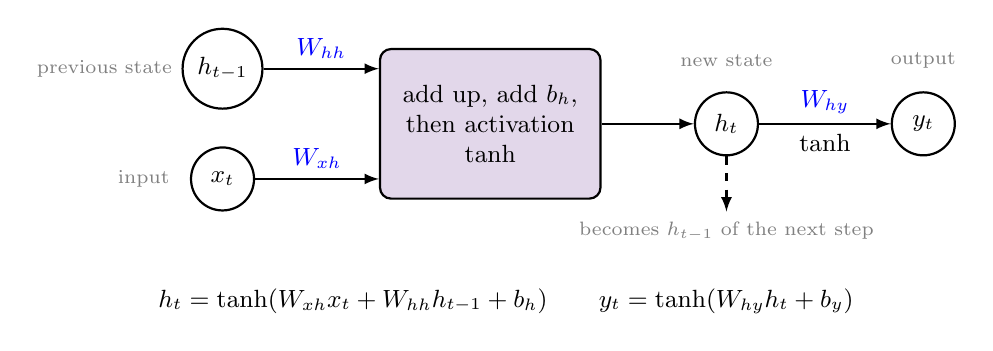
\begin{tikzpicture}[>=latex, thick, every node/.style={font=\small}]
\node[draw, circle, minimum size=8mm] (hp) at (0,1.1) {$h_{t-1}$};
\node[draw, circle, minimum size=8mm] (xt) at (0,-0.3) {$x_t$};
\node[font=\scriptsize, gray] at (-1.5,1.1) {previous state};
\node[font=\scriptsize, gray] at (-1.0,-0.3) {input};
\node[draw, rounded corners, fill=lightnyupurple!30, minimum width=2.8cm, minimum height=1.9cm, align=center] (cell) at (3.4,0.4) {add up, add $b_h$,\\then activation\\$\tanh$};
\node[draw, circle, minimum size=8mm] (ht) at (6.4,0.4) {$h_t$};
\node[draw, circle, minimum size=8mm] (yt) at (8.9,0.4) {$y_t$};
\node[font=\scriptsize, gray] at (6.4,1.2) {new state};
\node[font=\scriptsize, gray] at (8.9,1.2) {output};
\draw[->] (hp.east) -- node[above, blue] {$W_{hh}$} (cell.west |- hp.east);
\draw[->] (xt.east) -- node[above, blue] {$W_{xh}$} (cell.west |- xt.east);
\draw[->] (cell.east) -- (ht.west);
\draw[->] (ht.east) -- node[above, blue] {$W_{hy}$} node[below] {$\tanh$} (yt.west);
\draw[->, dashed] (ht.south) -- ++(0,-0.7) node[below, font=\scriptsize, gray] {becomes $h_{t-1}$ of the next step};
\node at (3.6,-1.85) {$h_t = \tanh(W_{xh}x_t + W_{hh}h_{t-1} + b_h) \qquad y_t = \tanh(W_{hy}h_t + b_y)$};
\end{tikzpicture}}
\end{center}
\end{frame}


%%%%%%%%%%%%%%%%%%%%%%%%%%%%%%%%%%%%%%%%%%%%%%%%%%%
\begin{frame}[fragile] \frametitle{RNN Types: Sequences In and Out}

RNN allow us to operate over sequences of vectors. Many types
\begin{center}
\includegraphics[width=0.8\linewidth,keepaspectratio]{rnn23}
\end{center}
Each rectangle is a vector and arrows represent functions (e.g. matrix multiply). Input vectors are in red, output vectors are in blue and green vectors hold the RNN's state (hidden layer nodes are called `state' here as it has memory)

\end{frame}

%%%%%%%%%%%%%%%%%%%%%%%%%%%%%%%%%%%%%%%%%%%%%%%%%%%
\begin{frame}[fragile] \frametitle{RNN as an ANN with a Loop}

\begin{center}
\includegraphics[width=0.8\linewidth,keepaspectratio]{rnn28}

\tiny{(Ref: RNN - Udacity)}

\end{center}

RNN can be imagined to be a usual ANN, with additional nodes from next layer back into inputs.
\end{frame}



% %%%%%%%%%%%%%%%%%%%%%%%%%%%%%%%%%%%%%%%%%%%%%%%%%%%
% \begin{frame}[fragile] \frametitle{What is RNN?}

% \begin{center}
% \includegraphics[width=0.8\linewidth,keepaspectratio]{rnn23}
% \end{center}
% One-to-One: Vanilla mode of processing without RNN, from fixed-sized input to fixed-sized output (e.g. image classification).
% \end{frame}

% %%%%%%%%%%%%%%%%%%%%%%%%%%%%%%%%%%%%%%%%%%%%%%%%%%%
% \begin{frame}[fragile] \frametitle{What is RNN?}

% \begin{center}
% \includegraphics[width=0.8\linewidth,keepaspectratio]{rnn23}
% \end{center}
% One-to-Many: Sequence output (e.g. image captioning takes an image (fixed size) and outputs a sentence of words).
% \end{frame}


% %%%%%%%%%%%%%%%%%%%%%%%%%%%%%%%%%%%%%%%%%%%%%%%%%%%
% \begin{frame}[fragile] \frametitle{Recurrent neural networks}
% \begin{center}
% \includegraphics[width=0.8\linewidth,keepaspectratio]{rnn23}
% \end{center}
% Many-to-One: Sequence input (e.g. sentiment analysis where a given sentence is classified as expressing positive or negative sentiment).
% \end{frame}

% %%%%%%%%%%%%%%%%%%%%%%%%%%%%%%%%%%%%%%%%%%%%%%%%%%%
% \begin{frame}[fragile] \frametitle{Recurrent neural networks}
% \begin{center}
% \includegraphics[width=0.8\linewidth,keepaspectratio]{rnn23}
% \end{center}
% Many-to-Many: Sequence input and sequence output (e.g. Machine Translation: an RNN reads a sentence in English and then outputs a sentence in French).
% \end{frame}

% % %%%%%%%%%%%%%%%%%%%%%%%%%%%%%%%%%%%%%%%%%%%%%%%%%%%
% % \begin{frame}[fragile] \frametitle{Recurrent neural networks}
% % \begin{center}
% % \includegraphics[width=0.8\linewidth,keepaspectratio]{rnn23}
% % \end{center}
% % Many-to-Many: Synced sequence input and output (e.g. video classification where we wish to label each frame of the video).
% % \end{frame}

% %%%%%%%%%%%%%%%%%%%%%%%%%%%%%%%%%%%%%%%%%%%%%%%%%%%
% \begin{frame}[fragile] \frametitle{Recurrent neural networks}
% \begin{center}
% \includegraphics[width=0.8\linewidth,keepaspectratio]{rnn23}
% \end{center}
% Notice that in every case are no pre-specified constraints on the lengths sequences because the recurrent transformation (green) is fixed and can be applied as many times as we like.
% \end{frame}



% %%%%%%%%%%%%%%%%%%%%%%%%%%%%%%%%%%%%%%%%%%%%%%%%%%%
% \begin{frame}[fragile] \frametitle{RNN: Sequential processing in absence of sequences.}
% \begin{center}
% \includegraphics[width=0.3\linewidth,keepaspectratio]{rnn24}
% \end{center}
% Images are fixed size. But for sequential numbers in it, RNN learns to read out house numbers from left to right.
% \end{frame}


%% http://karpathy.github.io/2015/05/21/rnn-effectiveness/
%% https://www.youtube.com/watch?v=iX5V1WpxxkY&index=10&list=LLsBKTrp45lTfHa_p49I2AEQ








% %%%%%%%%%%%%%%%%%%%%%%%%%%%%%%%%%%%%%%%%%%%%%%%%%%%
% \begin{frame}[fragile] \frametitle{RNNs Intuition}

% \begin{itemize}
% \item Human thoughts have persistence; humans don't start their thinking from scratch every second. 
% \item As you read this sentence, you understand each word based on your understanding of previous words.  
% \end{itemize}
% \end{frame}

% %%%%%%%%%%%%%%%%%%%%%%%%%%%%%%%%%%%%%%%%%%%%%%%%%%%
% \begin{frame}[fragile] \frametitle{RNNs Intuition}

% \begin{itemize}
% \item One of the appeals of RNNs is the idea that they are able to connect previous information to the present task
% \item E.g., using previous video frames to inform the understanding of the present frame.
% \item E.g., a language model tries to predict the next word based on the previous ones.
% \end{itemize}
% \end{frame}

% %%%%%%%%%%%%%%%%%%%%%%%%%%%%%%%%%%%%%%%%%%%%%%%%%%%
% \begin{frame}[fragile] \frametitle{What is Neural Memory?}

% \begin{itemize}
% \item List the alphabet forward\ldots. you can do it, yes?
% \item List the alphabet backward\ldots. hmmm\ldots perhaps a bit tougher.
% \item Try with the lyrics of a song you know?
% \item Why is it easier to recall forward than it is to recall backward? Can you jump into the middle of the second verse?\ldots hmm\ldots also difficult. Why?
% \end{itemize}
% \end{frame}

% %%%%%%%%%%%%%%%%%%%%%%%%%%%%%%%%%%%%%%%%%%%%%%%%%%%
% \begin{frame}[fragile] \frametitle{What is Neural Memory?}

% \begin{itemize}
% \item There's a very logical reason for this
% \item You learned them as a sequence. 
% \item You are really good at indexing from one letter to the next.
% \item It's a kind of conditional memory. (Once you given a start of poem, you can recite it further)
% \item All these  tasks are easier when you know what happened earlier in the sequence
% \end{itemize}
% \end{frame}

% %%%%%%%%%%%%%%%%%%%%%%%%%%%%%%%%%%%%%%%%%%%%%%%%%%%
% \begin{frame}[fragile] \frametitle{What is Neural Memory?}

% \begin{itemize}
% \item However, it's not that you don't have the song in your memory except when you're singing it. 
% \item Instead, when you try to jump straight to the middle of the song, you simply have a hard time finding that representation in your brain (perhaps that set of neurons).
% \item It starts searching all over looking for the middle of the song, but it hasn't tried to look for it this way before, so it doesn't have a map to the location of the middle of the second verse.
% \end{itemize}
% \end{frame}

%%%%%%%%%%%%%%%%%%%%%%%%%%%%%%%%%%%%%%%%%%%%%%%%%%%
\begin{frame}[fragile] \frametitle{One Step by Hand: The Cell}
\begin{itemize}
\item One hidden unit. The cell reads the new input $x_1$ and the old state $h_0$, and writes the new state $h_1$
\item $h_0 = 0$ is the starting state: the memory before anything is read. It is an input to step 1, not an output
\end{itemize}
\begin{center}
\adjustbox{max width=\linewidth}{%
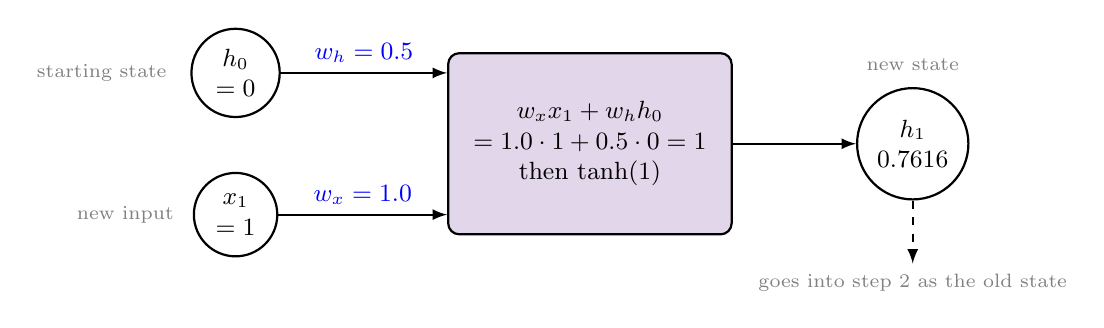
\begin{tikzpicture}[>=latex, thick, every node/.style={font=\small}]
\node[draw, circle, minimum size=10mm, align=center] (h0) at (0,1.3) {$h_0$\\$=0$};
\node[draw, circle, minimum size=10mm, align=center] (x1) at (0,-0.5) {$x_1$\\$=1$};
\node[font=\scriptsize, gray] at (-1.7,1.3) {starting state};
\node[font=\scriptsize, gray] at (-1.4,-0.5) {new input};
\node[draw, rounded corners, fill=lightnyupurple!30, minimum width=3.6cm, minimum height=2.3cm, align=center] (cell) at (4.5,0.4) {$w_x x_1 + w_h h_0$\\$= 1.0 \cdot 1 + 0.5 \cdot 0 = 1$\\then $\tanh(1)$};
\node[draw, circle, minimum size=12mm, align=center] (h1) at (8.6,0.4) {$h_1$\\$0.7616$};
\node[font=\scriptsize, gray] at (8.6,1.4) {new state};
\draw[->] (h0.east) -- node[above, blue] {$w_h = 0.5$} (cell.west |- h0.east);
\draw[->] (x1.east) -- node[above, blue] {$w_x = 1.0$} (cell.west |- x1.east);
\draw[->] (cell.east) -- (h1.west);
\draw[->, dashed] (h1.south) -- ++(0,-0.8) node[below, font=\scriptsize, gray] {goes into step 2 as the old state};
\end{tikzpicture}}
\end{center}
\end{frame}

%%%%%%%%%%%%%%%%%%%%%%%%%%%%%%%%%%%%%%%%%%%%%%%%%%%
\begin{frame}[fragile] \frametitle{One Step by Hand}
\begin{itemize}
\item One hidden unit, so everything fits on a slide: $h_t = \tanh(w_x x_t + w_h h_{t-1})$ with $w_x = 1.0$, $w_h = 0.5$ and $h_0 = 0$
\item Feed the sequence $x = (1, 0, 0)$
\end{itemize}
\begin{center}
\small
\adjustbox{max width=\linewidth}{%
\begin{tabular}{cccl}
\hline
Step & Input $x_t$ & Previous $h_{t-1}$ & New $h_t$ \\
\hline
1 & 1 & 0 & $\tanh(1 \cdot 1 + 0.5 \cdot 0) = 0.7616$ \\
2 & 0 & 0.7616 & $\tanh(0 + 0.5 \cdot 0.7616) = 0.3634$ \\
3 & 0 & 0.3634 & $\tanh(0 + 0.5 \cdot 0.3634) = 0.1797$ \\
\hline
\end{tabular}}
\end{center}
\begin{itemize}
\item The state carries the past forward: at step 3 there is no new input, yet $h_3$ is not 0
\item The $1$ from step 1 is still there, but it has shrunk from $0.7616$ to $0.1797$
\end{itemize}
\end{frame}

%%%%%%%%%%%%%%%%%%%%%%%%%%%%%%%%%%%%%%%%%%%%%%%%%%%
\begin{frame}[fragile] \frametitle{Order Changes the Answer}
\begin{center}
\small
\adjustbox{max width=\linewidth}{%
\begin{tabular}{ccc}
\hline
Sequence $(x_1, x_2, x_3)$ & Final state $h_3$ & Note \\
\hline
$(1, 0, 0)$ & 0.1797 & the 1 came first \\
$(0, 0, 1)$ & 0.7616 & the 1 came last \\
$(1, 1, 0)$ & 0.4141 & \\
$(0, 1, 1)$ & 0.8811 & \\
\hline
\end{tabular}}
\end{center}
\begin{itemize}
\item Same inputs, different order, different final state. A bag (a sum) would give the same number for $(1,0,0)$ and $(0,0,1)$
\item Recent inputs weigh more than old ones. This is useful for forecasting, and it is also the root of the fading problem later
\end{itemize}
\end{frame}

%%%%%%%%%%%%%%%%%%%%%%%%%%%%%%%%%%%%%%%%%%%%%%%%%%%
\begin{frame}[fragile] \frametitle{Same Weights at Every Step}
\begin{itemize}
% [upgrade-deck: rewritten 2026-10-26 | Task 5c | long bullets split into a lead plus sub-points; every fact kept; original below]
% \item With vectors, the same rule is $h_t = \tanh(W_{xh} x_t + W_{hh} h_{t-1} + b_h)$
% \item New here: $b_h$ is the \textbf{bias}, a vector of constants added before the $\tanh$, as in a dense layer. The one-unit example had none ($b_h = 0$). $W_{xh}$ and $W_{hh}$ are the weights $w_x$ and $w_h$ as matrices
% \item $W_{xh}$, $W_{hh}$ and $b_h$ are the same at step 1, step 2 and step 1000. Reading a longer sequence adds steps, not parameters
\item With vectors, the same rule is $h_t = \tanh(W_{xh} x_t + W_{hh} h_{t-1} + b_h)$
\item New here: $b_h$ is the \textbf{bias}, a vector of constants added before the $\tanh$, as in a dense layer
  \begin{itemize}
  \item The one-unit example had none ($b_h = 0$)
  \item $W_{xh}$ and $W_{hh}$ are the weights $w_x$ and $w_h$ as matrices
  \end{itemize}
\item $W_{xh}$, $W_{hh}$ and $b_h$ are the same at step 1, step 2 and step 1000
  \begin{itemize}
  \item Reading a longer sequence adds steps, not parameters
  \end{itemize}
\item Compare the CNN: one filter reused at every \emph{position} in space. The RNN reuses one set of weights at every \emph{step} in time
\item Training works on the unrolled copy and adds up the gradients of every use of the shared weights (back-propagation through time)
\end{itemize}
\end{frame}

%%%%%%%%%%%%%%%%%%%%%%%%%%%%%%%%%%%%%%%%%%%%%%%%%%%
\begin{frame}
  \begin{center}
    {\Large Memory in RNN}
  \end{center}
\end{frame}


% %%%%%%%%%%%%%%%%%%%%%%%%%%%%%%%%%%%%%%%%%%%%%%%%%%%
% \begin{frame}[fragile] \frametitle{What is Neural Memory?}

% \begin{itemize}
% \item If you wanted to train a neural network to predict whats the next scene would be in the next frame, it would be really helpful to know where the scene was in the last frame! 
% \item Sequential data like this is why we build recurrent neural networks.
% \end{itemize}
% \end{frame}

%%%%%%%%%%%%%%%%%%%%%%%%%%%%%%%%%%%%%%%%%%%%%%%%%%%
\begin{frame}[fragile] \frametitle{Neural Memory: The Plain Network}

\begin{itemize}
\item Neural networks have hidden layers. Normally, the state of your hidden layer is based ONLY on your input data. 
\item So, normally a neural network's information flow would look like this:
$input \rightarrow hidden  \rightarrow  output$
\item This is straightforward. Certain types of input create certain types of hidden layers. 
\item Certain types of hidden layers create certain types of output layers. 
\item It's kind-of a closed system. Memory changes this. 
\end{itemize}
\end{frame}


%%%%%%%%%%%%%%%%%%%%%%%%%%%%%%%%%%%%%%%%%%%%%%%%%%%
\begin{frame}[fragile] \frametitle{Neural Memory: Adding the Previous State}
\begin{itemize}
\item Memory means that the hidden layer is a combination of your input data at the current step and the hidden layer of the previous step.
$ (input + prev\_hidden) \rightarrow hidden \rightarrow output$
\item Why the hidden layer? Well, we could technically do this. 
$(input + prev\_input) \rightarrow hidden \rightarrow output$
\end{itemize}

\begin{center}
\includegraphics[width=0.8\linewidth,keepaspectratio]{rnn33}

{\tiny (Ref: Weights and Biases : Introduction to RNNs)}
\end{center}


\end{frame}

% %%%%%%%%%%%%%%%%%%%%%%%%%%%%%%%%%%%%%%%%%%%%%%%%%%%
% \begin{frame}[fragile] \frametitle{What is Neural Memory?}
% Here, we have 4 timesteps of a recurrent neural network pulling information from the previous hidden layer.
% \begin{itemize}
% \item $(input + empty\_hidden) \rightarrow hidden \rightarrow output$
% \item $(input + prev\_hidden) \rightarrow hidden \rightarrow output$
% \item $(input + prev\_hidden) \rightarrow hidden \rightarrow output$
% \item $(input + prev\_hidden) \rightarrow hidden \rightarrow output$
% \end{itemize}
% \end{frame}

%%%%%%%%%%%%%%%%%%%%%%%%%%%%%%%%%%%%%%%%%%%%%%%%%%%
\begin{frame}[fragile] \frametitle{Neural Memory: The Cell Equations}
Each cell
\begin{itemize}
% [upgrade-deck: rewritten 2026-10-26 | Task 1 | tanh set as a function and X_t written x_t, as on the other frames; original below]
% \item $h_t = tanh(W_{hh}h_{t-1} + W_{xh}X_t + b_h)$
% \item $y_t = tanh(W_{hy}h_t + b_y)$
\item $h_t = \tanh(W_{hh}h_{t-1} + W_{xh}x_t + b_h)$
\item $y_t = \tanh(W_{hy}h_t + b_y)$
\item Back-propagation will adjust all the weights for all unrolled steps.
\end{itemize}


\begin{center}
\includegraphics[width=0.3\linewidth,keepaspectratio]{rnn35}

{\tiny (Ref: RNN with Keras: Understanding computations - Alexis Huet)}


\includegraphics[width=0.6\linewidth,keepaspectratio]{rnn31}
\end{center}
\end{frame}


%%%%%%%%%%%%%%%%%%%%%%%%%%%%%%%%%%%%%%%%%%%%%%%%%%%
% [upgrade-deck: rewritten 2026-10-18 | Task 1 | both equations were labelled h_t', and the second ignored the first layer; the figure rnn36 shows two stacked layers]
% \begin{frame}[fragile] \frametitle{RNN with 2 hidden layers or units}
% Each cell
% \begin{itemize}
% \item $h_t' = tanh(W_{hh}h_{t-1} + W_{xh}X_t + b_h)$
% \item $h_t' = tanh(W_{hh}'h_{t-1}' + W_{xh}'X_t + b_h')$
% \item $y_t = tanh(W_{hy}h_t' + b_y)$
\begin{frame}[fragile] \frametitle{RNN with 2 hidden layers}
\begin{columns}[T]
\begin{column}{0.56\textwidth}
Each cell
\begin{itemize}
% [upgrade-deck: rewritten 2026-10-26 | Task 1 | tanh set as a function and X_t written x_t, as on the other frames; original below]
% \item $h_t = tanh(W_{hh}h_{t-1} + W_{xh}X_t + b_h)$
% \item $h_t' = tanh(W_{hh}'h_{t-1}' + W_{xh}'h_t + b_h')$
% \item $y_t = tanh(W_{hy}h_t' + b_y)$
\item $h_t = \tanh(W_{hh}h_{t-1} + W_{xh}x_t + b_h)$
\item $h_t' = \tanh(W_{hh}'h_{t-1}' + W_{xh}'h_t + b_h')$
\item $y_t = \tanh(W_{hy}h_t' + b_y)$
\item The second layer reads the first layer's state $h_t$ in place of the raw input.
\item Back-propagation will adjust all the weights for all unrolled steps.
\end{itemize}
\end{column}
\begin{column}{0.4\textwidth}
\begin{center}
\includegraphics[width=\linewidth,height=0.6\textheight,keepaspectratio]{rnn36}

{\tiny (Ref: RNN with Keras: Understanding computations - Alexis Huet)}
\end{center}
\end{column}
\end{columns}
\end{frame}

%%%%%%%%%%%%%%%%%%%%%%%%%%%%%%%%%%%%%%%%%%%%%%%%%%%
\begin{frame}[fragile] \frametitle{GRU cell}
\begin{columns}[T]
\begin{column}{0.56\textwidth}
Each cell
\begin{align*}
z_t =& \sigma(W_{zx} x_t + W_{zh} h_{t-1} + b_z) \\
r_t =& \sigma(W_{rx} x_t + W_{rh} h_{t-1} + b_r) \\
\tilde{h}_t =& \tanh(W_{ox} x_t + W_{oh} r_t h_{t-1} + b_o) \\
 \\
h_t =& z_t h_{t-1} + (1 - z_t) \tilde{h}_t
\end{align*} %]]>
\end{column}
\begin{column}{0.4\textwidth}
\begin{center}
\includegraphics[width=\linewidth,height=0.6\textheight,keepaspectratio]{rnn37}

{\tiny (Ref: RNN with Keras: Understanding computations - Alexis Huet)}
\end{center}
\end{column}
\end{columns}
\end{frame}

%%%%%%%%%%%%%%%%%%%%%%%%%%%%%%%%%%%%%%%%%%%%%%%%%%%
\begin{frame}[fragile] \frametitle{LSTM cell}
\begin{columns}[T]
\begin{column}{0.56\textwidth}
Each cell
% <![CDATA[
\begin{align*}
i_t =& \sigma(W_{ix} x_t + W_{ih} h_{t-1} + b_i) \\
f_t =& \sigma(W_{fx} x_t + W_{fh} h_{t-1} + b_f) \\
\tilde{c}_t =& \tanh(W_{cx} x_t + W_{ch} h_{t-1} + b_c) \\
o_t =& \sigma(W_{ox} x_t + W_{oh} h_{t-1} + b_o) \\
 \\
c_t =& f_t c_{t-1} + i_t \tilde{c}_t \\
h_t =& o_t \tanh(c_t)
\end{align*} %]]>
\end{column}
\begin{column}{0.34\textwidth}
\begin{center}
\includegraphics[width=\linewidth,keepaspectratio]{rnn38}

{\tiny (Ref: RNN with Keras: Understanding computations - Alexis Huet)}
\end{center}
\end{column}
\end{columns}
\end{frame}

%%%%%%%%%%%%%%%%%%%%%%%%%%%%%%%%%%%%%%%%%%%%%%%%%%%
% [Moved 2026-10-26 | Task 3 | from the start of dl_rnn_temperature_case_study.tex; it explains the LSTM cell above]
\begin{frame}[fragile]\frametitle{Reading the Gates of an LSTM}
\begin{itemize}
\item The memory $c_t$ is a running tally; three gates control it
\item Each gate is a number between 0 and 1 for every memory slot
\item Forget gate $f_t$: how much of the old memory to keep
\item Input gate $i_t$: how much of the new candidate $\tilde{c}_t$ to write
\item Output gate $o_t$: how much of the memory to show as the output $h_t$
\item $c_t = f_t c_{t-1} + i_t \tilde{c}_t$ keeps part of the old and adds part of the new
\item A GRU does the same job with two gates and no separate memory
\end{itemize}
\end{frame}


% %%%%%%%%%%%%%%%%%%%%%%%%%%%%%%%%%%%%%%%%%%%%%%%%%%%
% \begin{frame}[fragile] \frametitle{What is Neural Memory?}
% Colored show how hidden layer gets updated. 
% 4 timesteps with hidden layer recurrence:
% \begin{center}
% \includegraphics[width=0.6\linewidth,keepaspectratio]{rnn1}
% \end{center}
% 4 timesteps with input  layer recurrence:
% \begin{center}
% \includegraphics[width=0.6\linewidth,keepaspectratio]{rnn2}
% \end{center}
% Focus on the last hidden layer (4th line).
% \end{frame}

% %%%%%%%%%%%%%%%%%%%%%%%%%%%%%%%%%%%%%%%%%%%%%%%%%%%
% \begin{frame}[fragile] \frametitle{What is Neural Memory?}
% \begin{itemize}
% \item  In the hidden layer recurrence, we see a presence of every input seen so far. In the input layer recurrence, it's exclusively defined by the current and previous inputs. 
% \item This is why we model hidden recurrence.
% \item Hidden recurrence learns what to remember whereas input recurrence is hard wired to just remember the immediately previous datapoint. 
% \end{itemize}
% \end{frame}

% %%%%%%%%%%%%%%%%%%%%%%%%%%%%%%%%%%%%%%%%%%%%%%%%%%%
% \begin{frame}[fragile] \frametitle{What is Neural Memory?}
% \begin{itemize}
% \item  Now compare and contrast these two approaches with the backwards alphabet and middle-of-song exercises. 
% \item The hidden layer is constantly changing as it gets more inputs. 
% \item Furthermore, the only way that we could reach these hidden states is with the correct sequence of inputs.
% \end{itemize}
% \end{frame}



% %%%%%%%%%%%%%%%%%%%%%%%%%%%%%%%%%%%%%%%%%%%%%%%%%%%
% \begin{frame}[fragile] \frametitle{What is Neural Memory?}
% \begin{itemize}
% \item  What's the practical difference? Let's say we were trying to predict the next word in a song given the previous. 
% \item The ``input layer recurrence'' would break down if the song accidentally had the same sequence of two words in multiple places. 
% \item Think about it, if the song had the statements ''I love you'', and ''I love carrots'', and the network was trying to predict the next word, how would it know what follows ''I love''? 
% It could be carrots. It could be you. The network REALLY needs to know more about what part of the song its in.
% \end{itemize}
% \end{frame}


% %%%%%%%%%%%%%%%%%%%%%%%%%%%%%%%%%%%%%%%%%%%%%%%%%%%
% \begin{frame}[fragile] \frametitle{What is Neural Memory?}
% \begin{itemize}
% \item  It could be carrots. 
% \item It could be you. 
% \item The network REALLY needs to know more about what part of the song its in.
% \item However, the ''hidden layer recurrence'' doesn't break down in this way. 
% \item It subtely remembers everything it saw (with memories becoming more subtle as it they fade into the past).
% \end{itemize}
% \end{frame}


% %%%%%%%%%%%%%%%%%%%%%%%%%%%%%%%%%%%%%%%%%%%%%%%%%%%
% \begin{frame}[fragile] \frametitle{RNN - Neural Network Memory}
% Normal NN process:
% \begin{itemize}
% \item Our input layer to the neural network is determined by our input dataset. 
% \item Each row of input data is used to generate the hidden layer (via forward propagation). 
% \item Each hidden layer is then used to populate the output layer (assuming only 1 hidden layer)
% \end{itemize}
% \end{frame}


% %%%%%%%%%%%%%%%%%%%%%%%%%%%%%%%%%%%%%%%%%%%%%%%%%%%
% \begin{frame}[fragile] \frametitle{RNN - Neural Network Memory}
% \begin{itemize}
% \item Just saw, memory means that the hidden layer is a combination of the input data and the previous hidden layer. 
% \item How is this done?
% \item Much like every other propagation in neural networks, it's done with a matrix. 
% \item This matrix defines the relationship between the previous hidden layer and the current one.
% \end{itemize}
% \end{frame}

% %%%
% %%%%%%%%%%%%%%%%%%%%%%%%%%%%%%%%%%%%%%%%%%%%%%%%%%%%%%
% %%%\begin{frame}[fragile] \frametitle{RNN - Neural Network Memory}
% %%%\begin{center}
% %%%\includegraphics[width=0.6\linewidth,keepaspectratio]{rnn3}
% %%%\end{center}
% %%%\begin{itemize}
% %%%\item SYNAPSE\_0 propagates the input data to the hidden layer. 
% %%%\item SYNAPSE\_1 propagates the hidden layer to the output data. 
% %%%\item The new matrix (SYNAPSE\_h, the recurrent one), propagates from the hidden layer (layer\_1) to the hidden layer at the next timestep (still layer\_1). 
% %%%\end{itemize}
% %%%\end{frame}

% %%%%%%%%%%%%%%%%%%%%%%%%%%%%%%%%%%%%%%%%%%%%%%%%%%%
% \begin{frame}
  % \begin{center}
    % {\Large Graphical view of RNN}
  % \end{center}
% \end{frame}


% %%%%%%%%%%%%%%%%%%%%%%%%%%%%%%%%%%%%%%%%%%%%%%%%%%%
% \begin{frame}[fragile] \frametitle{RNN in Steps}
% \begin{center}
% \includegraphics[width=0.6\linewidth,keepaspectratio]{rnn4}
% \end{center}
% \begin{itemize}
% \item It depicts 4 timesteps. 
% \item The first is exclusively influenced by the input data. 
% \item The second one is a mixture of the first and second inputs. 
% \item This continues on. 
% \end{itemize}
% \end{frame}

% %%%%%%%%%%%%%%%%%%%%%%%%%%%%%%%%%%%%%%%%%%%%%%%%%%%
% \begin{frame}[fragile] \frametitle{RNN in Steps}
% \begin{center}
% \includegraphics[width=0.6\linewidth,keepaspectratio]{rnn4}
% \end{center}
% \begin{itemize}
% \item You should recognize that, in some way, network 4 is ''full''. 
% \item Presumably, timestep 5 would have to choose which memories to keep and which ones to overwrite. 
% \item It's the notion of memory ''capacity''. As you might expect, bigger layers can hold more memories for a longer period of time.
% \end{itemize}
% \end{frame}

% %%%%%%%%%%%%%%%%%%%%%%%%%%%%%%%%%%%%%%%%%%%%%%%%%%%
% \begin{frame}[fragile] \frametitle{RNN in Steps}
% \begin{center}
% \includegraphics[width=0.6\linewidth,keepaspectratio]{rnn4}
% \end{center}
% \begin{itemize}
% \item Also, this is when the network learns to forget irrelevant memories and remember important memories. 
% \item What significant thing do you notice in timestep 3? 
% \item Why is there more green in the hidden layer than the other colors?
% \end{itemize}
% \end{frame}

% %%%%%%%%%%%%%%%%%%%%%%%%%%%%%%%%%%%%%%%%%%%%%%%%%%%
% \begin{frame}[fragile] \frametitle{RNN in Steps}
% \begin{itemize}
% \item Also notice that the hidden layer is the barrier between the input and the output. 
% \item In reality, the output is no longer a pure function of the input. 
% \item The input is just changing what's in the memory, 
% \item and the output is exclusively based on the memory. 
% \end{itemize}
% \end{frame}

% %%%%%%%%%%%%%%%%%%%%%%%%%%%%%%%%%%%%%%%%%%%%%%%%%%%
% \begin{frame}[fragile] \frametitle{RNN in Steps}
% \begin{center}
% \includegraphics[width=0.6\linewidth,keepaspectratio]{rnn4}
% \end{center}
% \begin{itemize}
% \item Another interesting takeaway. 
% \item If there was no input at timesteps 2,3,and 4, the hidden layer would still change from timestep to timestep. 
% \end{itemize}
% \end{frame}

% %%%%%%%%%%%%%%%%%%%%%%%%%%%%%%%%%%%%%%%%%%%%%%%%%%%
% \begin{frame}[fragile] \frametitle{RNN in Steps}

% Back-propagation Through Time

% \begin{center}
% \includegraphics[width=0.6\linewidth,keepaspectratio]{rnn5}
% \end{center}
% \begin{itemize}
% \item So, how do recurrent neural networks learn? 
% \item Errors are bright yellow, derivatives are mustard colored.
% \item Picture shows back propagation coming from 4th step upto 3rd.
% \end{itemize}
% \end{frame}

% %%%%%%%%%%%%%%%%%%%%%%%%%%%%%%%%%%%%%%%%%%%%%%%%%%%
% \begin{frame}[fragile] \frametitle{RNN in Steps}
% \begin{center}
% \includegraphics[width=0.6\linewidth,keepaspectratio]{rnn5}
% \end{center}
% \begin{itemize}
% \item They learn by fully propagating forward from 1 to 4 and then back-propagating all the derivatives from 4 back to 1. 
% \item Its normal neural network, except that we're re-using the same weights (synapses 0,1,and h) in their respective places. 
% \end{itemize}
% \end{frame}


%%%%%%%%%%%%%%%%%%%%%%%%%%%%%%%%%%%%%%%%%%%%%%%%%%%%%
%%\begin{frame}[fragile] \frametitle{Recurrent neural networks}
%%
%%\begin{itemize}
%%\item Recurrent Neural Networks are networks with loops in them, allowing information to persist.
%%\item In the above diagram, a chunk of neural network, A, looks at some input xt and outputs a value ht. 
%%\item A loop allows information to be passed from one step of the network to the next. 
%%\end{itemize}
%%\end{frame}


%%%%%%%%%%%%%%%%%%%%%%%%%%%%%%%%%%%%%%%%%%%%%%%%%%%
% [Optional cut 2026-10-19 | DLCoEP trim for a one-hour session | restore by uncommenting this block]
% \begin{frame}
%   \begin{center}
%     {\Large Implementation of RNN}
%   \end{center}
% \end{frame}

%%%%%%%%%%%%%%%%%%%%%%%%%%%%%%%%%%%%%%%%%%%%%%%%%%%
% [Optional cut 2026-10-19 | DLCoEP trim for a one-hour session | restore by uncommenting this block]
% \begin{frame}[fragile] \frametitle{RNN Inputs Specification}
% FIXED sequence length case: Say,
% \begin{itemize}
% \item Dataset has 10000 rows and 64 features/columns
% \item Need to generate classification model, binary, so labels are 0 or 1.
% \item How does RNN handle this matrix (i.e., (10000,64))? Does it input each column something like this figure?
% \item Should SimpleRNN() units always be equal to the number of features?
% \end{itemize}
% 
% \begin{center}
% \includegraphics[width=0.2\linewidth,keepaspectratio]{rnn32}
% \end{center}
% 
% 
% \end{frame}

%%%%%%%%%%%%%%%%%%%%%%%%%%%%%%%%%%%%%%%%%%%%%%%%%%%
% [Optional cut 2026-10-19 | DLCoEP trim for a one-hour session | restore by uncommenting this block]
% \begin{frame}[fragile] \frametitle{RNN Inputs Specification}
% \begin{itemize}
% \item batch\_input\_shape to be with shape: \lstinline|(batch_size, X.shape[1], 1)|
% \item So batch size* 1000 examples will go at a time. Total, 10 such batches.
% \item Each of the 1000 example contains \lstinline|X.shape[1]| time-stamps (number of pink boxes in your image, same as number of features, ie 64) and each time-stamp is shape 1 (scalar). Dimensionality of that entity is 1. It can be a vector as well.
% \item So input shape is \lstinline|(1000,64,1)|
% \item The larger a batch, the more representative the computed gradient is for the whole data set, but larger memory requirements
% \end{itemize}
% 
% {\tiny (More info: https://stats.stackexchange.com/questions/153531/what-is-batch-size-in-neural-network)}
% 
% \end{frame}

%%%%%%%%%%%%%%%%%%%%%%%%%%%%%%%%%%%%%%%%%%%%%%%%%%%
% [Optional cut 2026-10-19 | DLCoEP trim for a one-hour session | restore by uncommenting this block]
% \begin{frame}[fragile] \frametitle{RNN Inputs Specification: Batch Size, Num Steps}
% \begin{itemize}
% \item `batch size' pertains to the amount of training samples to consider at a time for updating your network weights. Training can be erratic if weights are updated for each row. After a training pass of size batch\_size, the gradient of your loss function with respect to each of the network parameters is computed and your weights updated.
% \item Till the batch is over, losses per training sample are either averaged or accumulated, with that values, weights are updated. {\tiny (Ref: https://stats.stackexchange.com/questions/174708/how-are-weights-updated-in-the-batch-learning-method-in-neural-networks)}
% 
% \item In RNN, it is computationally very, very expensive to calculate the gradients of the loss function with respect to network parameters if you have to consider back-propagation through all states since the creation of your network, there is a neat little trick to speed up your computation: approximate your gradients with a subset of historical network states num\_steps.
% \end{itemize}
% 
% \begin{center}
% \includegraphics[width=0.2\linewidth,keepaspectratio]{rnn32}
% \end{center}
% 
% {\tiny (More info: https://stackoverflow.com/questions/44381450/doubts-regarding-batch-size-and-time-steps-in-rnn)}
% 
% \end{frame}


%%%%%%%%%%%%%%%%%%%%%%%%%%%%%%%%%%%%%%%%%%%%%%%%%%%
% [Optional cut 2026-10-19 | DLCoEP trim for a one-hour session | restore by uncommenting this block]
% \begin{frame}[fragile] \frametitle{RNN Inputs Specification: Batch Size, Num Steps}
% [upgrade-deck: commented out 2026-10-18 | Task 1 | 100 examples in batches of 5 give 20 updates per epoch, not 30]
% Example: data size of 100; batch size of 5, for 30 network parameter updates during each epoch.
% Example: data size of 100; batch size of 5, for 20 network parameter updates during each epoch.
% \begin{itemize}
% \item Propagates the first 5 training examples, updates its parameters based on the optimization method provided, then takes the next 5, until it made a full pass over the data. 
% \item num\_steps determines the amount of cells you unroll and hence the amount of data used in gradient computation. 
% \item As each cell/layer shares parameters, this does not result in an increase in parameters to optimize, but it enables context learning, which is why you'd want RNNs in the first place
% \end{itemize}
% So, NUM STEPS is the number of `features' you LOOK BACK (in case of text-words input) or consider while computing gradients and updating the weights.
% 
% \begin{center}
% \includegraphics[width=0.2\linewidth,keepaspectratio]{rnn32}
% \end{center}
% 
% {\tiny (More info: https://stackoverflow.com/questions/44381450/doubts-regarding-batch-size-and-time-steps-in-rnn)}
% 
% \end{frame}


%%%%%%%%%%%%%%%%%%%%%%%%%%%%%%%%%%%%%%%%%%%%%%%%%%%
% [Optional cut 2026-10-19 | DLCoEP trim for a one-hour session | restore by uncommenting this block]
% \begin{frame}[fragile] \frametitle{RNN LAYER Specification}
% RNN Layer can have multiple hidden states, physically but internally to the cell. Each physical RNN cell (called units) unrolls time-step wise.
% 
% \begin{itemize}
% \item Do we have to have RNN units, ie green, boxes, sames as number of columns or features, ie 64. %Green boxes are just time-step wise rolling, ie looping.
% \item No! units will be your output dim. Thats inside direction, its about number of internal state values, which are given as outputs as well as hidden states passed to the next time-step.
% \item This is ``\ldots to MANY'' architecture, for predicting next $n$ outputs.
% \item Units will be the shape of the RNN's internal states.
% \item So, if you declare units=2000 your output will be (1000,2000).)
% \item Each weight matrix will be num features x num outputs.
% \item Each output will get tuned, optimized as per its given output label.
% \item More units, is better to model the function. In case you want singular output you can still have more units and then later, add a dense layer to reduce the dimension to 1.
% \end{itemize}
% 
% \begin{center}
% \includegraphics[width=0.8\linewidth,keepaspectratio]{rnn34}
% 
% {\tiny (Ref: Weights and Biases : Introduction to RNNs)}
% 
% \end{center}
% 
% 
% \end{frame}

%%%%%%%%%%%%%%%%%%%%%%%%%%%%%%%%%%%%%%%%%%%%%%%%%%%
% [Optional cut 2026-10-19 | DLCoEP trim for a one-hour session | restore by uncommenting this block]
% \begin{frame}[fragile] \frametitle{RNN LAYER Specification}
% RNN Layer can have multiple hidden states, physically but internally to the cell. Each physical RNN cell (called units) unrolls time-step wise.
% 
% \begin{itemize}
% \item Do we have to have RNN units, ie green, boxes, sames as number of columns or features, ie 64. %Green boxes are just time-step wise rolling, ie looping.
% \item No! units will be your output dim. Thats inside direction, its about number of internal state values, which are given as outputs as well as hidden states passed to the next time-step.
% \item This is '\ldots to MANY" architecture, for predicting next $n$ outputs.
% \item Units will be the shape of the RNN's internal states. 
% \item So, if you declare units=2000 your output will be (1000,2000).
% \item Each weight matrix will be num features x num outputs.
% \item Each output will get tuned, optimized as per its given output label.
% \item More units, is better to model the function. In case you want singular output you can still have more units and then later, add a dense layer to reduce the dimension to 1.
% \end{itemize}
% 
% \begin{center}
% \includegraphics[width=0.8\linewidth,keepaspectratio]{rnn34}
% 
% {\tiny (Ref: Weights and Biases : Introduction to RNNs)}
% 
% \end{center}
% 
% 
% \end{frame}


%%%%%%%%%%%%%%%%%%%%%%%%%%%%%%%%%%%%%%%%%%%%%%%%%%%
% [Optional cut 2026-10-19 | DLCoEP trim for a one-hour session | restore by uncommenting this block]
% \begin{frame}[fragile] \frametitle{RNN Inputs Specification}
% VARIABLE sequence length case: Say,
% \begin{itemize}
% \item Can either PAD the sequence with '0's and make it FIXED size, for each batch (or overall), else specify 'None' for that variable for time steps in Keras.  If you don't want `0' padding, then you can specify sample weights. 
% \item Now, suppose length of training examples in
% \begin{align*}
% batch-1 &= 10, \\
% batch-2 &= 15. \\
% batch-3 &= 18 \ldots
% \end{align*}
% \item Now while training batch-1 , RNN will be unrolled/looped 10 times. For batch-2, 15 times and so on. The number of weights do not change, or even the network architecture does not change, but just the times same architecture is looped, changes in each batch.
% \end{itemize}
% 
% {\tiny (Ref: https://datascience.stackexchange.com/questions/26366/training-an-rnn-with-examples-of-different-lengths-in-keras)}.
% 
% 
% \end{frame}


%%%%%%%%%%%%%%%%%%%%%%%%%%%%%%%%%%%%%%%%%%%%%%%%%%%
% [Optional cut 2026-10-19 | DLCoEP trim for a one-hour session | restore by uncommenting this block]
% \begin{frame}[fragile] \frametitle{RNN Inputs Specification}
% \begin{itemize}
% 
% \item But, within a batch, do we need same fixed length of all sequences?
% \item Because Tensorflow (or any other framework) works on tensors/arrays and those can't be "ragged" like $[[1,2,3],[4,5]]$. 
% \item They need to be rectangular. Thats why within a batch, it needs to be fixed size. 
% \item Anyway achieved by num steps parameter, it extends or truncates. 
% \item The reason a fixed length is used in keras, is because it greatly improves performance by creating tensors of fixed shapes. 
% \item But that's only for training. After training, you'll have learned the right weights for your task.
% \end{itemize}
% 
% {\tiny (Ref: https://datascience.stackexchange.com/questions/26366/training-an-rnn-with-examples-of-different-lengths-in-keras)}.
% \begin{center}
% \includegraphics[width=0.2\linewidth,keepaspectratio]{rnn32}
% \end{center}
% 
% 
% \end{frame}


%%%%%%%%%%%%%%%%%%%%%%%%%%%%%%%%%%%%%%%%%%%%%%%%%%%
% [upgrade-deck: rewritten 2026-10-18 | Task 1 | binary cross-entropy needs a 0 to 1 output; the last line of the listing was: model.add(Dense(1, activation='relu'))]
% [Optional cut 2026-10-19 | DLCoEP trim for a one-hour session | restore by uncommenting this block]
% \begin{frame}[fragile] \frametitle{RNN Model}
% Code:
% \begin{lstlisting}
% X = X.reshape((X.shape[0], X.shape[1], 1)) # IT HAS TO BE 3D, so fake 1 dim added
% tr_X, ts_X, tr_y, ts_y = train_test_split(X, y, train_size=.8)
% batch_size = 1000
% 
% model = Sequential()
% model.add(SimpleRNN(64, activation='relu', batch_input_shape=(batch_size, X.shape[1], 1)))
% model.add(Dense(1, activation='sigmoid'))
% 
% model.compile(loss='binary_crossentropy', optimizer='adam', metrics=['accuracy'])
% 
% model.fit(tr_X, tr_y,
%           batch_size=batch_size, epochs=1,
%           shuffle=True, validation_data=(ts_X, ts_y))
% \end{lstlisting}
% 
% 
% 
% \end{frame}

%%%%%%%%%%%%%%%%%%%%%%%%%%%%%%%%%%%%%%%%%%%%%%%%%%%
% [Optional cut 2026-10-19 | DLCoEP trim for a one-hour session | restore by uncommenting this block]
% \begin{frame}[fragile] \frametitle{RNN Parameters calculations}
% 
% \begin{itemize}
% \item num\_units = equals the number of units in the RNN
% \item num\_features = equals the number features of your input
% \item input\_weights = num\_features*num\_units
% \item recurrent\_weights = num\_units*num\_units
% \item biases = num\_units*1
% \item total params = recurrent\_weights + input\_weights + biases
% \end{itemize}
% 
% \begin{center}
% \includegraphics[width=0.2\linewidth,keepaspectratio]{rnn32}
% \end{center}
% 
% 
% \end{frame}

%%%%%%%%%%%%%%%%%%%%%%%%%%%%%%%%%%%%%%%%%%%%%%%%%%%
% [Optional cut 2026-10-19 | DLCoEP trim for a one-hour session | restore by uncommenting this block]
% \begin{frame}[fragile] \frametitle{RNNs Model Summary}
% \begin{lstlisting}
% Layer (type)                 Output Shape              Param #   
% =================================================================
% simple_rnn_1 (SimpleRNN)     (1000, 64)                4224      
% _________________________________________________________________
% dense_1 (Dense)              (1000, 1)                 65        
% =================================================================
% Total params: 4,289
% Trainable params: 4,289
% Non-trainable params: 0
% _________________________________________________________________
% \end{lstlisting}
% 
% 
% \begin{center}
% \includegraphics[width=0.2\linewidth,keepaspectratio]{rnn32}
% \end{center}
% 
% 
% \end{frame}





%%%%%%%%%%%%%%%%%%%%%%%%%%%%%%%%%%%%%%%%%%%%%%%%%%%
\begin{frame}
  \begin{center}
    {\Large Strengths, Limits and Remedies}
  \end{center}
\end{frame}


%%%%%%%%%%%%%%%%%%%%%%%%%%%%%%%%%%%%%%%%%%%%%%%%%%%
\begin{frame}[fragile] \frametitle{RNN Advantages: The Fixed-Size Limit}

\begin{itemize}
\item The applications of standard Neural Networks (and also Convolutional Networks) are limited due to:
\item They only accepted a fixed-size vector as input (e.g., an image) and produce a fixed-size vector as output (e.g., probabilities of different classes). 
\item These models use a fixed amount of computational steps (e.g. the number of layers in the model).
\end{itemize}
\end{frame}


%%%%%%%%%%%%%%%%%%%%%%%%%%%%%%%%%%%%%%%%%%%%%%%%%%%
\begin{frame}[fragile] \frametitle{RNN Advantages: Sequences of Vectors}

\begin{itemize}
\item Recurrent Neural Networks are unique as they allow us to operate over sequences of vectors.
\item Sequences in the input, the output, or in the most general case both
\end{itemize}
\end{frame}


%%%
%%%
%%%
%%%
%%%%%%%%%%%%%%%%%%%%%%%%%%%%%%%%%%%%%%%%%%%%%%%%%%%%%%
%%%\begin{frame}[fragile] \frametitle{Stateful models}
%%%
%%%
%%%\begin{itemize}
%%%\item Using this idea, we can think of variable width inputs
%%%such that each new word simply updates our current prediction.
%%%In this way an RNN has two types of data inside of it:
%%%\begin{itemize}
%%%\item fixed weights, just as we have been using with CNNs
%%%\item stateful variables that are updated as it observes words
%%%in a document
%%%\end{itemize}
%%%\item Can also think of this as giving `memory' to the neural
%%%network.
%%%\end{itemize}
%%%\end{frame}
%%%
%%%
%%%
%%%%%%%%%%%%%%%%%%%%%%%%%%%%%%%%%%%%%%%%%%%%%%%%%%%%%%
%%%\begin{frame}[fragile] \frametitle{RNNs Memory}
%%%\begin{center}
%%%\includegraphics[width=0.8\linewidth,keepaspectratio]{rnnmem}
%%%\end{center}
%%%\end{frame}
%%%
%%%
%%%
%%%%%%%%%%%%%%%%%%%%%%%%%%%%%%%%%%%%%%%%%%%%%%%%%%%%%%
%%%\begin{frame}[fragile] \frametitle{}
%%%
%%%
%%%
%%%A third way of thinking about recurrent neural networks is to
%%%think of a network that has a loop in it. However, the self-input
%%%get's applied the \textit{next} time it is called.
%%%
%%%\begin{center}
%%%\includegraphics[width=0.3\linewidth,keepaspectratio]{cloah01.png}
%%%\end{center}
%%%
%%%\end{frame}
%%%
%%%%%%%%%%%%%%%%%%%%%%%%%%%%%%%%%%%%%%%%%%%%%%%%%%%%%%
%%%\begin{frame}[fragile] \frametitle{}
%%%
%%%A fourth way of thinking about a recurrent neural network is
%%%mathematically. We now have two parts to the update function
%%%in the RNN:
%%%\begin{align*}
%%%h_{t} &= {W x_t + b} + {U h_{t-1}}
%%%\end{align*}
%%%Notice that $U$ must always be a square matrix,
%%%because we could unravel this one time further to yield:
%%%\begin{align*}
%%%h_{t} &= W x_t + b + U W x_{t-1} + U b + U^2 h_{t-2}
%%%\end{align*}
%%%
%%%\end{frame}
%%%
%%%%%%%%%%%%%%%%%%%%%%%%%%%%%%%%%%%%%%%%%%%%%%%%%%%%%%
%%%\begin{frame}[fragile] \frametitle{What's different?}
%%%\begin{itemize}
%%%\item At each time step, output of hidden layers $H$ are added back for the next input.
%%%\item Outputs are also calculated at each time step ($Y_t$)
%%%\item Same wts and biases are shared across iterations
%%%\item Its like a state machine cell (remembering something)
%%%\item Can be used for sequences
%%%\end{itemize}
%%%
%%%
%%%\end{frame}
%%%
%%%%%%%%%%%%%%%%%%%%%%%%%%%%%%%%%%%%%%%%%%%%%%%%%%%%%%
%%%\begin{frame}[fragile] \frametitle{What's different?}
%%%\begin{center}
%%%\includegraphics[width=0.8\linewidth,keepaspectratio]{rnnwts}
%%%\end{center}
%%%
%%%\end{frame}
%%%
%%%
%%%
%%%%%%%%%%%%%%%%%%%%%%%%%%%%%%%%%%%%%%%%%%%%%%%%%%%%%%
%%%\begin{frame}[fragile] \frametitle{RNN}
%%%
%%%\begin{center}
%%%\includegraphics[width=0.8\linewidth,keepaspectratio]{rnnsamewts}
%%%\end{center}
%%%Output $y^i$ depends on $x_1, x_2,\ldots x_i$
%%%
%%%\end{frame}
%%%
%%%%%%%%%%%%%%%%%%%%%%%%%%%%%%%%%%%%%%%%%%%%%%%%%%%%%%
%%%\begin{frame}[fragile] \frametitle{On Sequences}
%%%
%%%
%%%\begin{itemize}
%%%\item Each cell, gets input, does iterations to try to match with given outputs. In the process, calculates wts and biases, as usual. May not work. 
%%%\item Instead of one cell, have a series and see if $Y_5$ can be forced.
%%%\item It is achieved by backpropagating through all cells, backwards.
%%%\item All $H$''s are adjusted, so $W$''s and $b$''s
%%%\item Can train on sequence of characters and verify open and close brackets
%%%\end{itemize}
%%%\begin{center}
%%%\includegraphics[width=0.8\linewidth,keepaspectratio]{rnnseq}
%%%\end{center}
%%%
%%%\end{frame}
%%%
%%%%%%%%%%%%%%%%%%%%%%%%%%%%%%%%%%%%%%%%%%%%%%%%%%%%%%
%%%\begin{frame}[fragile] \frametitle{How to train RNN?}
%%%
%%%\begin{center}
%%%\includegraphics[width=0.8\linewidth,keepaspectratio]{rnntrain}
%%%\end{center}
%%%Find the network parameters to minimize the total cost
%%%
%%%\end{frame}
%%%
%%%
%%%
%%%%%%%%%%%%%%%%%%%%%%%%%%%%%%%%%%%%%%%%%%%%%%%%%%%%%%
%%%\begin{frame}[fragile] \frametitle{Of course it can be deep}
%%%\begin{center}
%%%\includegraphics[width=0.8\linewidth,keepaspectratio]{rnndeep}
%%%\end{center}
%%%\end{frame}
%%%
%%%%%%%%%%%%%%%%%%%%%%%%%%%%%%%%%%%%%%%%%%%%%%%%%%%%%%
%%%\begin{frame}[fragile] \frametitle{Bidirectional RNN}
%%%\begin{center}
%%%\includegraphics[width=\linewidth,keepaspectratio]{rnnbi}
%%%\end{center}
%%%\end{frame}
%%%
%%%%%%%%%%%%%%%%%%%%%%%%%%%%%%%%%%%%%%%%%%%%%%%%%%%%%%
%%%\begin{frame}[fragile] \frametitle{Bidirectional RNN}
%%%\begin{center}
%%%\includegraphics[width=\linewidth,keepaspectratio]{rnnbi}
%%%\end{center}
%%%\end{frame}
%%%
%%%
%%%%%%%%%%%%%%%%%%%%%%%%%%%%%%%%%%%%%%%%%%%%%%%%%%%%%%
%%%\begin{frame}[fragile] \frametitle{Many to Many (Output is shorter)}
%%%Both input and output are both sequences, but the output is shorter.
%%%E.g. Speech Recognition
%%%\begin{center}
%%%\includegraphics[width=\linewidth,keepaspectratio]{rnnmm}
%%%\end{center}
%%%\end{frame}
%%%
%%%%%%%%%%%%%%%%%%%%%%%%%%%%%%%%%%%%%%%%%%%%%%%%%%%%%%
%%%\begin{frame}[fragile] \frametitle{Can also Stack them}
%%%\begin{center}
%%%\includegraphics[width=\linewidth,keepaspectratio]{rnnstack}
%%%\end{center}
%%%\end{frame}
%%%
%%%%%%%%%%%%%%%%%%%%%%%%%%%%%%%%%%%%%%%%%%%%%%%%%%%%%%
%%%\begin{frame}[fragile] \frametitle{RNN Types a summary}
%%%Input vectors are in red, output vectors are in blue and green vectors hold the RNN's state
%%%\begin{center}
%%%\includegraphics[width=\linewidth,keepaspectratio]{rnntypes}
%%%\end{center}
%%%
%%%\end{frame}
%%%
%%%%%%%%%%%%%%%%%%%%%%%%%%%%%%%%%%%%%%%%%%%%%%%%%%%%%%
%%%\begin{frame}[fragile] \frametitle{RNN Types a summary}
%%%\begin{itemize}
%%%\item Standard mode of processing without RNN, from fixed-sized input to fixed-sized output (e.g. image classification). 
%%%\item Sequence output (e.g. image captioning takes an image and outputs a sentence of words). 
%%%\item Sequence input (e.g. sentiment analysis where a given sentence is classified as expressing positive or negative sentiment). 
%%%\item Sequence input and sequence output (e.g. Machine Translation: an RNN reads a sentence in English and then outputs a sentence in French). 
%%%\item Synced sequence input and output (e.g. video classification where we wish to label each frame of the video).
%%%\end{itemize}
%%%\end{frame}
%%%
%%%%%%%%%%%%%%%%%%%%%%%%%%%%%%%%%%%%%%%%%%%%%%%%%%%%%%
%%%\begin{frame}[fragile] \frametitle{RNN Apps}
%%%\begin{center}
%%%\includegraphics[width=\linewidth,keepaspectratio]{rnnapps}
%%%\end{center}
%%%\end{frame}
%%%
%%%%%%%%%%%%%%%%%%%%%%%%%%%%%%%%%%%%%%%%%%%%%%%%%%%%%%
%%%\begin{frame}[fragile] \frametitle{Name Entity Recognition}
%%%Detecting named entities like name of people, locations, organization, etc. in a sentence.
%%%\begin{center}
%%%\includegraphics[width=\linewidth,keepaspectratio]{rnnner}
%%%\end{center}
%%%\end{frame}
%%%
%%%%%%%%%%%%%%%%%%%%%%%%%%%%%%%%%%%%%%%%%%%%%%%%%%%%%%
%%%\begin{frame}[fragile] \frametitle{Name Entity Recognition}
%%%\begin{center}
%%%\includegraphics[width=\linewidth,keepaspectratio]{rnnnerlayer}
%%%\end{center}
%%%\end{frame}
%%%
%%%%%%%%%%%%%%%%%%%%%%%%%%%%%%%%%%%%%%%%%%%%%%%%%%%%%%
%%%\begin{frame}[fragile] \frametitle{Unfortunately}
%%%RNN-based network is not always easy to learn
%%%\begin{center}
%%%\includegraphics[width=\linewidth,keepaspectratio]{rnndisadv}
%%%\end{center}
%%%\end{frame}
%%%
%%%%%%%%%%%%%%%%%%%%%%%%%%%%%%%%%%%%%%%%%%%%%%%%%%%%%%
%%%\begin{frame}[fragile] \frametitle{Errors}
%%%The error surface is rough.
%%%\begin{center}
%%%\includegraphics[width=\linewidth,keepaspectratio]{rnnerr}
%%%\end{center}
%%%\end{frame}
%%%
%%%
%%%%%%%%%%%%%%%%%%%%%%%%%%%%%%%%%%%%%%%%%%%%%%%%%%%%%%
%%%\begin{frame}[fragile] \frametitle{Anything better}
%%%\begin{itemize}
%%%\item ``Michael was born in Paris.<sentences> His mother tongue is ''
%%%\item Clue is far away. You need to have very long chain of such cells. That's limitation.
%%%\item Just few words is ok.
%%%\item Solution: LSTM (Long Short Term Memory)
%%%\end{itemize}
%%%\end{frame}
%%%
%%%
%%%%%%%%%%%%%%%%%%%%%%%%%%%%%%%%%%%%%%%%%%%%%%%%%%%%%%
%%%\begin{frame}[fragile] \frametitle{Anything better}
%%%\begin{center}
%%%\includegraphics[width=\linewidth,keepaspectratio]{rnn2lstm}
%%%\end{center}
%%%\end{frame}



% %%%%%%%%%%%%%%%%%%%%%%%%%%%%%%%%%%%%%%%%%%%%%%%%%%%
% \begin{frame}
  % \begin{center}
    % {\Large RNN variations}
    
    % LSTM-GRU
  % \end{center}
% \end{frame}

% %%%%%%%%%%%%%%%%%%%%%%%%%%%%%%%%%%%%%%%%%%%%%%%%%%%
% \begin{frame}[fragile] \frametitle{Recap: Simple RNN}
% \begin{center}
% \includegraphics[width=0.5\linewidth,keepaspectratio]{lstm49}

% \tiny{(Ref: Intro to Deep Learning - Coursera, National Research University Higher School of Economics)}
% \end{center}
% RNN takes previous hidden state ($h_{t-1}$), current input ($x_t$) and generates new/next hidden state ($h_t$) by formula $h_t = f_h ( Vx_t + Wh_{t-1} + b_h)$
% \end{frame}

%%%%%%%%%%%%%%%%%%%%%%%%%%%%%%%%%%%%%%%%%%%%%%%%%%%
\begin{frame}[fragile] \frametitle{RNN Shortcomings}
\begin{itemize}
\item RNN does not work in some situations
\item Especially when long past words need to be accounted for
\item Due to Vanishing Gradient problem.
\end{itemize}

\begin{center}
\includegraphics[width=\linewidth,keepaspectratio]{rnn42}
\end{center}
\end{frame}

%%%%%%%%%%%%%%%%%%%%%%%%%%%%%%%%%%%%%%%%%%%%%%%%%%%
\begin{frame}[fragile] \frametitle{RNN vanishing gradients}
\begin{itemize}
% [upgrade-deck: rewritten 2026-10-18 | Task 1 | a linear hidden function is not a fix for vanishing gradients, and "further layers" should read earlier time steps; original bullets kept below]
% \item Vanilla RNNs suffers at vanishing gradients problems.
% \item A modest recurrent neural network may have 200-to-400 input time steps, resulting conceptually in a very deep network.
% \item problem: The derivative the activation nonlinearities, sigmoid or tanh, is smaller
% than 1. So, after some timesteps, very minute gradient remains to make any weight changes. In further layers, weights do not change. So, NO TRAINING.
% \item Solution: the hidden transfer function should be a linear function. Relu (rectilinear activation function) looks and acts like a linear function, making it easier to train and less likely to saturate, but is, in fact, a nonlinear function. The ReLU derivative is a constant of either 0 or 1, so it isn’t as likely to suffer from vanishing gradients.
% [upgrade-deck: rewritten 2026-10-26 | Task 5c | long bullets split into a lead plus sub-points; every fact kept; original below]
% \item Vanilla RNNs suffer from the vanishing gradient problem.
% \item A modest recurrent neural network may have 200 to 400 input time steps, resulting conceptually in a very deep network.
% \item Problem: back-propagation through time multiplies the gradient at every step by the derivative of the activation (at most 1 for tanh, at most 0.25 for sigmoid) and by the recurrent weights. If these factors are below 1, the product shrinks toward zero.
% \item So the early time steps get almost no gradient, their weights barely change, and long-range dependencies are not learned.
% \item Remedies: gated cells (LSTM, GRU) are the standard fix. ReLU helps because its derivative is 0 or 1, but it can make gradients explode; gradient clipping handles that.
\item Vanilla RNNs suffer from the vanishing gradient problem
\item A modest RNN may have 200 to 400 input steps: conceptually a very deep network
\item \textbf{Problem:} back-propagation through time multiplies the gradient at every step
  \begin{itemize}
  \item By the derivative of the activation: at most 1 for tanh, at most 0.25 for sigmoid
  \item And by the recurrent weights. If these factors are below 1, the product shrinks toward zero
  \end{itemize}
\item So the early steps get almost no gradient, their weights barely change, and long-range dependencies are not learned
\item \textbf{Remedies:} gated cells (LSTM, GRU) are the standard fix
  \begin{itemize}
  \item ReLU helps (its derivative is 0 or 1) but can make gradients explode
  \item Gradient clipping handles that
  \end{itemize}
\end{itemize}

\begin{center}
\includegraphics[width=0.8\linewidth,keepaspectratio]{rnn46}
\end{center}
\end{frame}

%%%%%%%%%%%%%%%%%%%%%%%%%%%%%%%%%%%%%%%%%%%%%%%%%%%
\begin{frame}[fragile] \frametitle{Fading by Numbers}
\begin{center}
\small
\adjustbox{max width=\linewidth}{%
\begin{tabular}{rc}
\hline
Steps $T$ & $|\partial h_T / \partial x_1|$, plain tanh RNN \\
\hline
5 & $2.11 \times 10^{-2}$ \\
10 & $1.25 \times 10^{-3}$ \\
20 & $6.09 \times 10^{-6}$ \\
40 & $4.72 \times 10^{-11}$ \\
80 & $3.31 \times 10^{-21}$ \\
\hline
\end{tabular}}
\end{center}
\begin{itemize}
\item How much the very first input still moves the last hidden state. Untrained layer, default start, 32 units, median of 20 random starts
\item Each extra step multiplies by a factor below 1, so the effect shrinks exponentially: at 80 steps the first input is, for the network, gone
\item Caution: with the same default start, a GRU and an LSTM also fade in this test (about $10^{-17}$ at 80 steps). Gates give the network a way to hold information after training, not a free pass at the start
\end{itemize}
\end{frame}

%%%%%%%%%%%%%%%%%%%%%%%%%%%%%%%%%%%%%%%%%%%%%%%%%%%
\begin{frame}[fragile] \frametitle{How LSTM Eases Vanishing Gradient}
\begin{itemize}
% [upgrade-deck: rewritten 2026-10-26 | Task 1 | "solves" overclaims: the previous slide shows a GRU or LSTM also fades at the untrained start; original below]
% \item LSTM increases memory network, handles more information, longer memory.
% \item LSTM network has three gates that update and control the cell states.
% \item So if we want Gradient not to vanish, our network needs to increase the likelihood that at least some of these sub gradients will not vanish.
% \item Forget gate sub-gradient does not behave similarly with other sub-gradient, so they all do not converge to zero.
\item An LSTM adds a cell state $c_t$: a separate memory that carries information across many steps
\item Three gates update and control the cell state
\item The cell state changes by addition, $c_t = f_t c_{t-1} + i_t \tilde{c}_t$
\item The gradient to earlier steps is a sum of several parts. We want at least some of them not to vanish
\item The forget-gate part does not shrink the way the other parts do, so they do not all go to zero
\item Gates ease the problem; they do not remove it. At the untrained start a GRU or an LSTM also fades (previous slide)
\end{itemize}

{\tiny (Ref: How LSTM networks solve the problem of vanishing gradients
- Nir Arbel)}

\end{frame}

%%%%%%%%%%%%%%%%%%%%%%%%%%%%%%%%%%%%%%%%%%%%%%%%%%%
\begin{frame}[fragile] \frametitle{One Vector per Sequence: Three Readouts}
\begin{itemize}
% [upgrade-deck: rewritten 2026-10-26 | Task 5c | long bullets split into a lead plus sub-points; every fact kept; original below]
% \item For a sentiment label or a fault class we need one vector for the whole sequence, then a classifier on top. Three common ways to get it:
% \item \textbf{Last state} $h_T$: simple, but the whole sequence is squeezed through one vector. Order is not lost, but old information has faded (recency bias)
% \item \textbf{Pooling over time}: keep every $h_t$ and take the mean or the maximum of each feature over all steps. An early, strong signal survives
% \item \textbf{Attention}: keep every $h_t$ and let the model learn how much each step counts for this decision
% \item A fourth, orthogonal fix is to read the sequence in both directions (next slides)
\item A sentiment label or a fault class needs one vector for the whole sequence, then a classifier on top. Three common ways:
\item \textbf{Last state} $h_T$: simple, but the whole sequence is squeezed through one vector
  \begin{itemize}
  \item Order is not lost, but old information has faded (recency bias: the newest steps dominate)
  \end{itemize}
\item \textbf{Pooling over time}: take the mean or the maximum of each feature over all the $h_t$. An early, strong signal survives
\item \textbf{Attention}: let the model learn how much each $h_t$ counts for this decision
\item A fourth, separate fix: read the sequence in both directions (next slides)
\end{itemize}
\begin{center}
\adjustbox{max width=\linewidth, max totalheight=0.28\textheight}{%
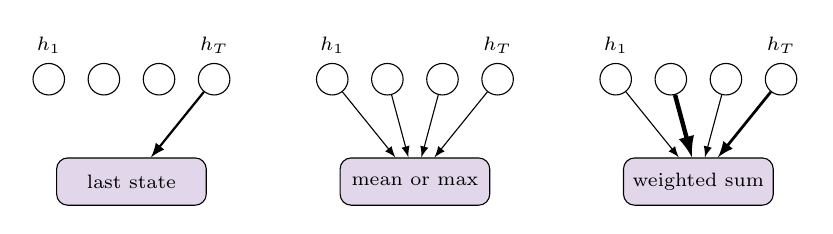
\begin{tikzpicture}[>=latex, every node/.style={font=\scriptsize}, st/.style={draw, circle, minimum size=4mm, inner sep=0pt}, bx/.style={draw, rounded corners, fill=lightnyupurple!30, minimum width=19mm, minimum height=6mm}]
\begin{scope}
\foreach \i/\x in {1/0, 2/0.7, 3/1.4, 4/2.1} \node[st] (a\i) at (\x,0) {};
\node[anchor=south] at (a1.north) {$h_1$};
\node[anchor=south] at (a4.north) {$h_T$};
\node[bx] (ab) at (1.05,-1.3) {last state};
\draw[->, thick] (a4) -- (ab);
\end{scope}
\begin{scope}[xshift=3.6cm]
\foreach \i/\x in {1/0, 2/0.7, 3/1.4, 4/2.1} \node[st] (b\i) at (\x,0) {};
\node[anchor=south] at (b1.north) {$h_1$};
\node[anchor=south] at (b4.north) {$h_T$};
\node[bx] (bb) at (1.05,-1.3) {mean or max};
\foreach \i in {1,2,3,4} \draw[->] (b\i) -- (bb);
\end{scope}
\begin{scope}[xshift=7.2cm]
\foreach \i/\x in {1/0, 2/0.7, 3/1.4, 4/2.1} \node[st] (c\i) at (\x,0) {};
\node[anchor=south] at (c1.north) {$h_1$};
\node[anchor=south] at (c4.north) {$h_T$};
\node[bx] (cb) at (1.05,-1.3) {weighted sum};
\draw[->, line width=0.4pt] (c1) -- (cb);
\draw[->, line width=1.6pt] (c2) -- (cb);
\draw[->, line width=0.4pt] (c3) -- (cb);
\draw[->, line width=1.0pt] (c4) -- (cb);
\end{scope}
\end{tikzpicture}}

{\tiny Thicker arrow, larger share. Last state uses one step; pooling treats all steps alike; attention learns the shares.}
\end{center}
\end{frame}

%%%%%%%%%%%%%%%%%%%%%%%%%%%%%%%%%%%%%%%%%%%%%%%%%%%
\begin{frame}[fragile] \frametitle{Early Evidence: Which Readout Works?}
\begin{itemize}
\item Task: sequences of 60 steps of noise; the label is whether a $+3$ marker sits in steps 1 to 3. Chance is 50\%. One run each
\end{itemize}
\begin{center}
\small
\adjustbox{max width=\linewidth}{%
\begin{tabular}{lrc}
\hline
Model & Parameters & Test accuracy \\
\hline
Plain RNN, last state & 338 & 85.3\% \\
Plain RNN, mean over time & 338 & 90.4\% \\
Plain RNN, max over time & 338 & 99.2\% \\
Plain RNN, bidirectional & 674 & 99.1\% \\
GRU, max over time & 946 & 99.3\% \\
GRU, bidirectional & 1,890 & 99.2\% \\
GRU, last state (100 epochs) & 946 & 52.2\% \\
LSTM, last state (100 epochs) & 1,250 & 50.9\% \\
\hline
\end{tabular}}
\end{center}
\begin{itemize}
% [upgrade-deck: rewritten 2026-10-26 | Task 5c | long bullets split into a lead plus sub-points; every fact kept; original below]
% \item Max pooling brings the early marker straight to the classifier. Bidirectional works because the backward pass ends at step 1, where the marker is fresh
% \item The last-state GRU and LSTM did not learn this task in our training budget, while the plain RNN did partly. We do not claim a ranking of cell types from one synthetic run
\item \textbf{Max pooling:} brings the early marker straight to the classifier
\item \textbf{Bidirectional:} the backward pass ends at step 1, where the marker is fresh
\item The last-state GRU and LSTM did not learn this task in our training budget, while the plain RNN did partly
\item We do not claim a ranking of cell types from one synthetic run
\end{itemize}
\end{frame}

%%%%%%%%%%%%%%%%%%%%%%%%%%%%%%%%%%%%%%%%%%%%%%%%%%%
\begin{frame}[fragile] \frametitle{Bidirectional RNN}
\begin{center}
\adjustbox{max width=0.7\linewidth, max totalheight=0.40\textheight}{\includegraphics{rnnbi}}
\end{center}
\begin{itemize}
\item Two recurrent layers: one reads left to right, one right to left. At each step their states are joined, so every step has context from both sides
\item The cost is twice the parameters (338 became 674 in the test before) and the whole sequence must be available
\item Fine for classifying a finished recording or sentence. Not possible for real-time forecasting, where the future has not happened yet
\end{itemize}
\end{frame}

%%%%%%%%%%%%%%%%%%%%%%%%%%%%%%%%%%%%%%%%%%%%%%%%%%%
% [upgrade-deck: rewritten 2026-10-26 | Tasks 5 and 5c | the definitions got their own frame with an Intuition callout; the worked example follows on the next frame; original below]
% \begin{frame}[fragile] \frametitle{Attention: A Weighted Look Back}
% \begin{itemize}
% \item Keep all hidden states $h_1, \dots, h_T$. Score each against a query $q$, turn scores into weights with softmax, and mix: $s_i = q \cdot h_i$, \quad $\alpha = \mathrm{softmax}(s)$, \quad $c = \sum_i \alpha_i h_i$
% \item Example: $h_1 = (1,0)$, $h_2 = (0,1)$, $h_3 = (1,1)$ and $q = (1,0)$
% \end{itemize}
\begin{frame}[fragile] \frametitle{Attention: A Weighted Look Back}
\begin{itemize}
\item Keep all hidden states $h_1, \dots, h_T$, not only the last one
\item \textbf{Score} each state against a query $q$ (a vector for what we are looking for): $s_i = q \cdot h_i$
\item \textbf{Weights:} softmax turns the scores into positive numbers that add up to 1: $\alpha = \mathrm{softmax}(s)$
\item \textbf{Mix} the states with those weights: $c = \sum_i \alpha_i h_i$
\end{itemize}
\begin{block}{Intuition}
Think of reading your notes with a highlighter. The query is the question you ask, the scores say which lines match it, and the weights decide how much of each line goes into your answer.
\end{block}
\end{frame}

%%%%%%%%%%%%%%%%%%%%%%%%%%%%%%%%%%%%%%%%%%%%%%%%%%%
\begin{frame}[fragile] \frametitle{Attention: A Worked Example}
\begin{itemize}
\item Example: $h_1 = (1,0)$, $h_2 = (0,1)$, $h_3 = (1,1)$ and $q = (1,0)$
\end{itemize}
\begin{center}
\small
\adjustbox{max width=\linewidth}{%
\begin{tabular}{lccc}
\hline
 & $h_1$ & $h_2$ & $h_3$ \\
\hline
score $q \cdot h_i$ & 1 & 0 & 1 \\
weight $\alpha_i$ & 0.4223 & 0.1554 & 0.4223 \\
\hline
\end{tabular}}
\end{center}
\begin{itemize}
\item Context $c = 0.4223\,(1,0) + 0.1554\,(0,1) + 0.4223\,(1,1) = (0.8446,\ 0.5777)$
\item A plain average would give $(0.6667,\ 0.6667)$: attention leans toward the states that match the query
\end{itemize}
\end{frame}

%%%%%%%%%%%%%%%%%%%%%%%%%%%%%%%%%%%%%%%%%%%%%%%%%%%
\begin{frame}[fragile] \frametitle{Attention: The Road to Transformers}
\begin{itemize}
\item Attention was first added on top of RNNs to ease the one-vector bottleneck: the decision can look back at every step, not only the last one
\item A Transformer keeps attention and drops the recurrence. It adds position information so that order is not lost, and it reads all steps at once, which suits parallel hardware
\item That is a pointer, not part of this session: the point here is why the bottleneck mattered
\item Recurrent nets have not disappeared. Small, cheap models that process a stream one step at a time are still a good fit when memory and compute are tight
\end{itemize}
\end{frame}

%%%%%%%%%%%%%%%%%%%%%%%%%%%%%%%%%%%%%%%%%%%%%%%%%%%
\begin{frame}[fragile] \frametitle{Quick Check: Sequences}
\begin{block}{Think About It}
1. A sensor gives 8 readings per step, and a layer has 32 hidden units. The window grows from 100 to 1000 steps. What happens to the parameter count?
\begin{enumerate}
  \item[A.] Both a dense layer on the window and a recurrent layer grow about ten times.
  \item[B.] The dense layer grows about ten times; the recurrent layer stays the same.
  \item[C.] The recurrent layer grows about ten times; the dense layer stays the same.
  \item[D.] Both stay the same.
\end{enumerate}
2. In the early-marker task, which readout lifted a plain RNN from 85\% to about 99\%?
\begin{enumerate}
  \item[A.] Last state only.
  \item[B.] Max over time (or reading in both directions).
  \item[C.] More hidden units with the same last-state readout.
  \item[D.] Shuffling the steps.
\end{enumerate}
\end{block}
\end{frame}

%%%%%%%%%%%%%%%%%%%%%%%%%%%%%%%%%%%%%%%%%%%%%%%%%%%
\begin{frame}[fragile] \frametitle{Quick Check: Sequences}
\begin{block}{Answer}
\textbf{1. Correct: B.} The dense layer on the window has $T \times 8 \times 32$ weights plus biases: 25,632 at 100 steps and 256,032 at 1000. The recurrent layer reuses the same weights at every step: 1,344 for a plain RNN in both cases.

\textbf{2. Correct: B.} Max over time keeps the early marker's strong response, and a backward pass ends exactly at the early steps. We did not test C, and D destroys the order the label depends on.
\end{block}
\end{frame}

%%%%%%%%%%%%%%%%%%%%%%%%%%%%%%%%%%%%%%%%%%%%%%%%%%%
\begin{frame}[fragile] \frametitle{Summary}
\begin{itemize}
% [upgrade-deck: rewritten 2026-10-26 | Tasks 1 and 5c | grammar, "solve" overclaims (see Fading by Numbers), long bullet split; original below]
% \item RNNs suffer from vanishing gradients and caused by long series of multiplications of small values, diminishing the gradients and causing the learning process to become degenerate.
% \item LSTMs solve the problem using a unique additive gradient structure that includes direct access to the forget gate’s activations, enabling the network to encourage desired behaviour from the error gradient using frequent gates update on every time step of the learning process.
\item RNNs suffer from vanishing gradients, caused by long series of multiplications of small values
  \begin{itemize}
  \item The gradient shrinks, and the early steps barely learn
  \end{itemize}
\item LSTMs ease the problem with an additive gradient structure
  \begin{itemize}
  \item It gives direct access to the forget gate's activations
  \item Gates are updated at every step, so the network can encourage the desired behaviour from the error gradient
  \end{itemize}
\item Gates help, but they do not remove the problem: at the untrained start a GRU or an LSTM also fades
\item To get one vector from a sequence: last state, pooling over time, attention, or both directions
\end{itemize}

{\tiny (Ref: How LSTM networks solve the problem of vanishing gradients
- Nir Arbel)}

\end{frame}


\subsection{GRU}
% Colours of the presentation template, defined here as well so that the TikZ diagrams also compile in the cheat sheet.
\definecolor{nyupurple}{RGB}{90, 35, 140}
\definecolor{lightnyupurple}{RGB}{159, 120, 184}

% GRU diagram, built in stages: #1 = 1 draws the update gate, #2 = 1 draws the reset gate.
\providecommand{\grudiagram}[2]{%
\adjustbox{max width=\linewidth, max totalheight=0.42\textheight}{%
\begin{tikzpicture}[>=latex, thick, every node/.style={font=\small}, st/.style={draw, circle, minimum size=9mm, inner sep=1pt}, gt/.style={draw, rounded corners, fill=orange!25, minimum height=7mm, align=center, inner sep=3pt}]
\node[st] (hp) at (0,2) {$h_{t-1}$};
\node[st] (xt) at (0,-0.25) {$x_t$};
\node[draw, rounded corners, fill=lightnyupurple!30, minimum width=26mm, minimum height=12mm, align=center] (cd) at (5,0) {candidate $\tilde{h}_t$\\$\tanh$};
\node[draw, rounded corners, fill=white, minimum width=11mm, minimum height=7mm] (bl) at (9,2) {mix};
\node[st] (ht) at (11.5,2) {$h_t$};
\node[font=\scriptsize, gray, above] at (hp.north) {previous state};
\node[font=\scriptsize, gray, below] at (xt.south) {input};
\node[font=\scriptsize, gray, above] at (ht.north) {new state};
\draw[->, line width=1.6pt, lightnyupurple!70!black] (hp) -- node[above, font=\scriptsize, black] {old memory, passed on} (bl);
\fill (2,2) circle (2pt);
\draw[->] (xt.east) -- (3.7,-0.25);
\ifnum#2=1
\node[gt] (rg) at (2,1.05) {reset\\$r_t$};
\draw (2,2) -- (rg.north);
\draw[->] (rg.south) -- (2,0.25) -- (3.7,0.25);
\else
\draw[->] (2,2) -- (2,0.25) -- (3.7,0.25);
\fi
\draw[->] (cd.east) -| node[pos=0.25, below, font=\scriptsize] {new content} (bl.south);
\ifnum#1=1
\node[gt] (zg) at (9,3.5) {update $z_t$};
\draw[->] (zg.south) -- (bl.north);
\fi
\draw[->] (bl) -- (ht);
\end{tikzpicture}}}

%%%%%%%%%%%%%%%%%%%%%%%%%%%%%%%%%%%%%%%%%%%%%%%%%%%
\begin{frame}
  \begin{center}
    {\Large Gated Recurrent Unit (GRU)}
  \end{center}
\end{frame}


%%%%%%%%%%%%%%%%%%%%%%%%%%%%%%%%%%%%%%%%%%%%%%%%%%%
\begin{frame}[fragile] \frametitle{Why Gates?}
\begin{itemize}
\item A plain RNN rewrites its whole state at every step: $h_t = \tanh(W_{xh}x_t + W_{hh}h_{t-1} + b_h)$
\item Nothing is copied unchanged: every old value passes through weights and a $\tanh$, step after step
\item So it cannot hold a value until it is needed, or ignore a useless reading such as a sensor glitch
\item A \textbf{gate} is a number between 0 and 1 for every memory slot (one component of the state vector)
  \begin{itemize}
  \item It comes from a sigmoid, a curve that squeezes any number into the range 0 to 1
  \item 0 blocks, 1 lets everything through, and in between lets a share through
  \end{itemize}
\item The GRU (Cho et al., 2014) uses gates so the cell can choose, step by step, between keeping and rewriting its memory
\end{itemize}
\begin{block}{Intuition}
A gate works like a tap on a pipe. Fully closed, nothing passes; fully open, everything passes. The network learns how far to open each tap at every step.
\end{block}
\end{frame}


%%%%%%%%%%%%%%%%%%%%%%%%%%%%%%%%%%%%%%%%%%%%%%%%%%%
\begin{frame}[fragile] \frametitle{The GRU Main Path}
\begin{center}
\grudiagram{0}{0}
\end{center}
\begin{itemize}
\item Same two inputs as a plain RNN: the old state $h_{t-1}$ and the new input $x_t$
\item The cell proposes a \textbf{candidate} $\tilde{h}_t$: what the new state could be
\item The new state is a \textbf{mix} of the old memory and the candidate
\item The old memory reaches the mix directly, with no weight matrix and no $\tanh$ on the way: a short path
\end{itemize}
\end{frame}


%%%%%%%%%%%%%%%%%%%%%%%%%%%%%%%%%%%%%%%%%%%%%%%%%%%
\begin{frame}[fragile] \frametitle{The Update Gate}
\begin{center}
\grudiagram{1}{0}
\end{center}
\begin{itemize}
\item The update gate decides the mix, one value per memory slot: $z_t = \sigma(W_{zx}x_t + W_{zh}h_{t-1} + b_z)$
\item $h_t = z_t \odot h_{t-1} + (1 - z_t) \odot \tilde{h}_t$, where $\odot$ is a slot-by-slot product
\item $z_t$ near 1 copies the old memory; $z_t$ near 0 replaces it with the candidate
\item One slot, $h_{t-1} = 0.8$ and candidate $-0.2$:
  \begin{itemize}
  \item $z_t = 0.9$ gives $0.9 \cdot 0.8 + 0.1 \cdot (-0.2) = 0.70$, mostly kept
  \item $z_t = 0.1$ gives $0.1 \cdot 0.8 + 0.9 \cdot (-0.2) = -0.10$, mostly replaced
  \end{itemize}
\end{itemize}
\end{frame}


%%%%%%%%%%%%%%%%%%%%%%%%%%%%%%%%%%%%%%%%%%%%%%%%%%%
\begin{frame}[fragile] \frametitle{The Reset Gate}
\begin{center}
\grudiagram{1}{1}
\end{center}
\begin{itemize}
\item The reset gate sits on the path from the old state into the candidate: $r_t = \sigma(W_{rx}x_t + W_{rh}h_{t-1} + b_r)$
\item Candidate: $\tilde{h}_t = \tanh(W_{cx}x_t + W_{ch}(r_t \odot h_{t-1}) + b_c)$
\item $r_t$ near 1: the candidate sees the full history, like a plain RNN cell
\item $r_t$ near 0: the candidate is built from the new input alone, a fresh start for the proposal
\item Two different jobs: the update gate decides how much to \emph{replace}; the reset gate decides what the proposal may \emph{look at}
\end{itemize}
\end{frame}


%%%%%%%%%%%%%%%%%%%%%%%%%%%%%%%%%%%%%%%%%%%%%%%%%%%
\begin{frame}[fragile] \frametitle{GRU in Equations}
\begin{align*}
z_t =& \sigma(W_{zx} x_t + W_{zh} h_{t-1} + b_z) \\
r_t =& \sigma(W_{rx} x_t + W_{rh} h_{t-1} + b_r) \\
\tilde{h}_t =& \tanh(W_{cx} x_t + W_{ch} (r_t \odot h_{t-1}) + b_c) \\
h_t =& z_t \odot h_{t-1} + (1 - z_t) \odot \tilde{h}_t
\end{align*}
\begin{itemize}
\item Three blocks of weights, each the size of a plain RNN's: about three times its parameters at the same width
\item One state is carried from step to step: $h_t$
\item As before, the same weights are used at every step
\end{itemize}
\end{frame}


%%%%%%%%%%%%%%%%%%%%%%%%%%%%%%%%%%%%%%%%%%%%%%%%%%%
\begin{frame}[fragile] \frametitle{What a GRU Gives and What Remains}
\textbf{Gives}
\begin{itemize}
\item Can hold a value across many steps: keep $z_t$ near 1
\item Can ignore an input, or restart its context with the reset gate
\item A short direct path for memory, and for the gradient on its way back
\item One state and fewer parameters than an LSTM: quick to train
\end{itemize}
\textbf{Still an issue}
\begin{itemize}
\item Memory and output are the same vector $h_t$: whatever is remembered is also shown
\item Keep and replace are tied: $z_t$ and $1 - z_t$ cannot be set separately
\item Gates ease the vanishing-gradient problem; they do not remove it
\item Still one step at a time, so very long sequences are slow
\end{itemize}
\end{frame}

\subsection{LSTM}
% Colours of the presentation template, defined here as well so that the TikZ diagrams also compile in the cheat sheet.
\definecolor{nyupurple}{RGB}{90, 35, 140}
\definecolor{lightnyupurple}{RGB}{159, 120, 184}

% LSTM diagram, built in stages: #1 = 1 shows the cell-state highway only, 2 adds the forget and input gates
% with the candidate, 3 adds the output gate. All gates read the same pair (h_{t-1}, x_t), drawn once as a bus.
\providecommand{\lstmdiagram}[1]{%
\adjustbox{max width=\linewidth, max totalheight=0.42\textheight}{%
\begin{tikzpicture}[>=latex, thick, every node/.style={font=\small}, st/.style={draw, circle, minimum size=9mm, inner sep=1pt}, gt/.style={draw, rounded corners, fill=orange!25, minimum width=11mm, minimum height=7mm, align=center, inner sep=2pt}, op/.style={draw, circle, minimum size=6mm, inner sep=0pt, fill=white}]
\node[st] (cp) at (0,3) {$c_{t-1}$};
\node[op] (fm) at (3,3) {$\times$};
\node[op] (ad) at (6,3) {$+$};
\node[st] (ct) at (11,3) {$c_t$};
\node[font=\scriptsize, gray, above] at (cp.north) {old memory};
\node[font=\scriptsize, gray, above] at (ct.north) {new memory};
\draw[->, line width=1.6pt, lightnyupurple!70!black] (cp) -- (fm);
\draw[->, line width=1.6pt, lightnyupurple!70!black] (fm) -- (ad);
\draw[->, line width=1.6pt, lightnyupurple!70!black] (ad) -- (ct);
\ifnum#1=1
\node[font=\scriptsize, above=3pt] at (fm.north) {scale down};
\node[font=\scriptsize, above=3pt] at (ad.north) {add};
\fi
\ifnum#1>1
\node[font=\scriptsize, above=3pt] at (fm.north) {erase};
\node[font=\scriptsize, above=3pt] at (ad.north) {write};
\node[draw, rounded corners, fill=white, minimum height=7mm] (bus) at (0,-0.4) {$h_{t-1},\ x_t$};
\draw[gray] (bus.east) -- (9,-0.4);
\node[gt] (fg) at (3,0.6) {forget\\$f_t$};
\node[gt] (ig) at (5,0.6) {input\\$i_t$};
\node[draw, rounded corners, fill=lightnyupurple!30, minimum width=11mm, minimum height=7mm, align=center, inner sep=2pt] (cg) at (7,0.6) {cand.\\$\tilde{c}_t$};
\node[op] (ml) at (6,1.9) {$\times$};
\draw[gray] (3,-0.4) -- (fg.south);
\draw[gray] (5,-0.4) -- (ig.south);
\draw[gray] (7,-0.4) -- (cg.south);
\draw[->] (fg.north) -- (fm.south);
\draw[->] (ig.north) -- (5,1.9) -- (ml.west);
\draw[->] (cg.north) -- (7,1.9) -- (ml.east);
\draw[->] (ml.north) -- (ad.south);
\fi
\ifnum#1>2
\node[gt] (og) at (9,0.6) {output\\$o_t$};
\draw[gray] (9,-0.4) -- (og.south);
\fill (8.2,3) circle (2pt);
\node[op, minimum size=8mm] (th) at (8.2,1.9) {$\tanh$};
\node[op] (mo) at (9,1.9) {$\times$};
\node[st] (ht) at (11,1.9) {$h_t$};
\node[font=\scriptsize, gray, below] at (ht.south) {output};
\draw[->] (8.2,3) -- (th.north);
\draw[->] (th.east) -- (mo.west);
\draw[->] (og.north) -- (mo.south);
\draw[->] (mo.east) -- (ht.west);
\fi
\end{tikzpicture}}}

%%%%%%%%%%%%%%%%%%%%%%%%%%%%%%%%%%%%%%%%%%%%%%%%%%%
\begin{frame}
  \begin{center}
    {\Large Long Short-Term Memory (LSTM)}
  \end{center}
\end{frame}


%%%%%%%%%%%%%%%%%%%%%%%%%%%%%%%%%%%%%%%%%%%%%%%%%%%
\begin{frame}[fragile] \frametitle{What an LSTM Adds}
\begin{itemize}
\item In a plain RNN or a GRU, one vector $h_t$ does two jobs: it is the memory and it is the output
\item The LSTM (Hochreiter and Schmidhuber, 1997) separates them
  \begin{itemize}
  \item \textbf{Cell state} $c_t$: the long-term memory, a conveyor belt that runs through time
  \item \textbf{Hidden state} $h_t$: what the cell shows at this step
  \end{itemize}
\item Three gates, each set on its own: \textbf{forget} (erase), \textbf{input} (write) and \textbf{output} (show)
\item The problem it targets: carrying information across a long gap, for example the number of load cycles since the last service, without every step's work overwriting it
\end{itemize}
\begin{block}{Intuition}
Think of a notebook and what you say aloud. The notebook (cell state) keeps what matters over a long time; what you say at each step (hidden state) is only the part of the notebook that is useful right now.
\end{block}
\end{frame}


%%%%%%%%%%%%%%%%%%%%%%%%%%%%%%%%%%%%%%%%%%%%%%%%%%%
\begin{frame}[fragile] \frametitle{The Cell-State Highway}
\begin{center}
\lstmdiagram{1}
\end{center}
\begin{itemize}
\item The memory $c_t$ runs along the top, from $c_{t-1}$ to $c_t$
\item It is changed at only two points: scaled down (erase), then added to (write)
\item No weight matrix and no $\tanh$ sits on this path, so information can ride it nearly unchanged
\end{itemize}
\end{frame}


%%%%%%%%%%%%%%%%%%%%%%%%%%%%%%%%%%%%%%%%%%%%%%%%%%%
\begin{frame}[fragile] \frametitle{Forget Gate, Input Gate and Candidate}
\begin{center}
\lstmdiagram{2}
\end{center}
\begin{itemize}
\item All of them read the same pair $(h_{t-1}, x_t)$, drawn once as the line at the bottom
\item $f_t = \sigma(W_{fx}x_t + W_{fh}h_{t-1} + b_f)$ is how much of the old memory to keep; $i_t = \sigma(W_{ix}x_t + W_{ih}h_{t-1} + b_i)$ is how much of the candidate to write
\item $\tilde{c}_t = \tanh(W_{cx}x_t + W_{ch}h_{t-1} + b_c)$ and $c_t = f_t \odot c_{t-1} + i_t \odot \tilde{c}_t$
\item One slot: $c_{t-1} = 2.0$, $f_t = 0.9$, $i_t = 0.5$, candidate $0.6$ gives $c_t = 0.9 \cdot 2.0 + 0.5 \cdot 0.6 = 2.1$
\end{itemize}
\end{frame}


%%%%%%%%%%%%%%%%%%%%%%%%%%%%%%%%%%%%%%%%%%%%%%%%%%%
\begin{frame}[fragile] \frametitle{The Output Gate}
\begin{center}
\lstmdiagram{3}
\end{center}
\begin{itemize}
\item $o_t = \sigma(W_{ox}x_t + W_{oh}h_{t-1} + b_o)$ and $h_t = o_t \odot \tanh(c_t)$
\item $\tanh$ squeezes the memory into $(-1, 1)$; the output gate decides how much of it to show
\item The cell can store a value now and reveal it only when it is needed
\item Same slot: $\tanh(2.1) = 0.9705$ and $o_t = 0.5$ give $h_t \approx 0.49$
\item Both $c_t$ and $h_t$ go to the next step; $h_t$ is also what the next layer sees
\end{itemize}
\end{frame}


%%%%%%%%%%%%%%%%%%%%%%%%%%%%%%%%%%%%%%%%%%%%%%%%%%%
\begin{frame}[fragile] \frametitle{LSTM and Vanishing Gradients}
\begin{itemize}
\item Along the cell-state path, the factor from one step to the previous one is the forget gate: $\partial c_t / \partial c_{t-1} = f_t$ (slot by slot)
\item In a plain RNN the factor involves $W_{hh}$ and the slope of $\tanh$, usually below 1: in the earlier test the first input's effect fell to about $10^{-21}$ after 80 steps
\item If the network learns $f_t \approx 0.99$, then over 50 steps about 61\% of the gradient survives ($0.99^{50} = 0.61$)
  \begin{itemize}
  \item With $f_t = 0.9$ only 0.5\% survives ($0.9^{50} = 0.005$): the gate must learn to stay near 1
  \end{itemize}
\item Gates ease the problem; they do not remove it
  \begin{itemize}
  \item At the untrained start a GRU and an LSTM also fade (about $10^{-17}$ at 80 steps, same test as the plain RNN)
  \item Gates give the network a way to hold information once trained, not a free pass at the start
  \end{itemize}
\end{itemize}

{\tiny (Ref: How LSTM networks solve the problem of vanishing gradients
- Nir Arbel)}

\end{frame}


%%%%%%%%%%%%%%%%%%%%%%%%%%%%%%%%%%%%%%%%%%%%%%%%%%%
\begin{frame}[fragile] \frametitle{What an LSTM Gives and What It Costs}
\textbf{Gives}
\begin{itemize}
\item Long-range memory held apart from the output
\item Separate control to erase, write and show
\item Well tested on many sequence tasks
\end{itemize}
\textbf{Costs}
\begin{itemize}
\item Four blocks of weights: about four times a plain RNN, against three for a GRU
\item Two states to carry, more computation, more to tune
\item Still one step at a time, and very long gaps remain hard
\item On small problems a GRU often does as well
\end{itemize}
\end{frame}


%%%%%%%%%%%%%%%%%%%%%%%%%%%%%%%%%%%%%%%%%%%%%%%%%%%
\begin{frame}[fragile] \frametitle{Plain RNN, GRU and LSTM Side by Side}
\begin{center}
\small
\adjustbox{max width=\linewidth}{%
\begin{tabular}{lccc}
\hline
 & Plain RNN & GRU & LSTM \\
\hline
States carried & 1 & 1 & 2 ($h_t$, $c_t$) \\
Gates & none & 2 & 3 \\
Weights, against a plain RNN & 1x & 3x & 4x \\
Keep and replace & no choice & tied, one gate & separate gates \\
Memory apart from output & no & no & yes \\
\hline
\end{tabular}}
\end{center}
\end{frame}


%%%%%%%%%%%%%%%%%%%%%%%%%%%%%%%%%%%%%%%%%%%%%%%%%%%
\begin{frame}[fragile]\frametitle{Quick Check: Gated Cells}
\begin{block}{Think About It}
1. In a GRU, the update gate $z_t$ is close to 1 for one memory slot. What happens to that slot?
\begin{enumerate}
  \item[A.] It is replaced by the candidate.
  \item[B.] It keeps its old value almost unchanged.
  \item[C.] It is set to zero.
  \item[D.] It is shown only to the next layer.
\end{enumerate}
2. What does an LSTM have that a GRU does not?
\begin{enumerate}
  \item[A.] Gates.
  \item[B.] A separate cell state, so memory is kept apart from the output.
  \item[C.] Immunity to vanishing gradients at the untrained start.
  \item[D.] Fewer parameters.
\end{enumerate}
\end{block}
\end{frame}

%%%%%%%%%%%%%%%%%%%%%%%%%%%%%%%%%%%%%%%%%%%%%%%%%%%
\begin{frame}[fragile]\frametitle{Quick Check: Gated Cells}
\begin{block}{Answer}
\textbf{1. Correct: B.} The new state is $z_t h_{t-1} + (1 - z_t)\tilde{h}_t$, so $z_t$ near 1 keeps the old value. A describes $z_t$ near 0.

\textbf{2. Correct: B.} A GRU has gates too (A), and at the untrained start both cells fade (C). An LSTM has more parameters, not fewer (D); its distinct feature is the separate cell state $c_t$.
\end{block}
\end{frame}

\subsection{Reading Out a Sequence}
% Moved 2026-10-28 from dl_rnn.tex: how to get one vector from a sequence, with any recurrent cell.
% Follows the plain RNN, GRU and LSTM sections (dl_rnn, dl_gru, dl_lstm).
%%%%%%%%%%%%%%%%%%%%%%%%%%%%%%%%%%%%%%%%%%%%%%%%%%%
\begin{frame}[fragile] \frametitle{One Vector per Sequence: Three Readouts}
\begin{itemize}
% [upgrade-deck: rewritten 2026-10-26 | Task 5c | long bullets split into a lead plus sub-points; every fact kept; original below]
% \item For a sentiment label or a fault class we need one vector for the whole sequence, then a classifier on top. Three common ways to get it:
% \item \textbf{Last state} $h_T$: simple, but the whole sequence is squeezed through one vector. Order is not lost, but old information has faded (recency bias)
% \item \textbf{Pooling over time}: keep every $h_t$ and take the mean or the maximum of each feature over all steps. An early, strong signal survives
% \item \textbf{Attention}: keep every $h_t$ and let the model learn how much each step counts for this decision
% \item A fourth, orthogonal fix is to read the sequence in both directions (next slides)
\item With a plain RNN, a GRU or an LSTM, a sentiment label or a fault class needs one vector for the whole sequence, then a classifier on top. Three common ways:
\item \textbf{Last state} $h_T$: simple, but the whole sequence is squeezed through one vector
  \begin{itemize}
  \item Order is not lost, but old information has faded (recency bias: the newest steps dominate)
  \end{itemize}
\item \textbf{Pooling over time}: take the mean or the maximum of each feature over all the $h_t$. An early, strong signal survives
\item \textbf{Attention}: let the model learn how much each $h_t$ counts for this decision
\item A fourth, separate fix: read the sequence in both directions (the Bidirectional RNN frame)
\end{itemize}
\begin{center}
\adjustbox{max width=\linewidth, max totalheight=0.28\textheight}{%
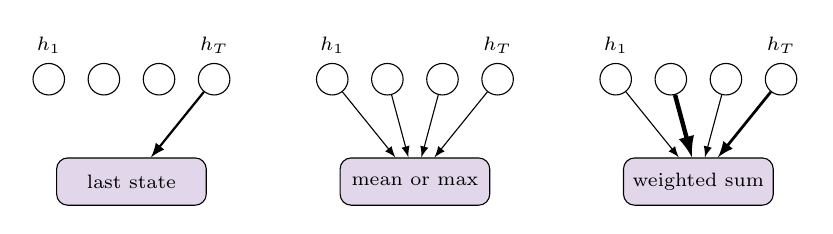
\begin{tikzpicture}[>=latex, every node/.style={font=\scriptsize}, st/.style={draw, circle, minimum size=4mm, inner sep=0pt}, bx/.style={draw, rounded corners, fill=lightnyupurple!30, minimum width=19mm, minimum height=6mm}]
\begin{scope}
\foreach \i/\x in {1/0, 2/0.7, 3/1.4, 4/2.1} \node[st] (a\i) at (\x,0) {};
\node[anchor=south] at (a1.north) {$h_1$};
\node[anchor=south] at (a4.north) {$h_T$};
\node[bx] (ab) at (1.05,-1.3) {last state};
\draw[->, thick] (a4) -- (ab);
\end{scope}
\begin{scope}[xshift=3.6cm]
\foreach \i/\x in {1/0, 2/0.7, 3/1.4, 4/2.1} \node[st] (b\i) at (\x,0) {};
\node[anchor=south] at (b1.north) {$h_1$};
\node[anchor=south] at (b4.north) {$h_T$};
\node[bx] (bb) at (1.05,-1.3) {mean or max};
\foreach \i in {1,2,3,4} \draw[->] (b\i) -- (bb);
\end{scope}
\begin{scope}[xshift=7.2cm]
\foreach \i/\x in {1/0, 2/0.7, 3/1.4, 4/2.1} \node[st] (c\i) at (\x,0) {};
\node[anchor=south] at (c1.north) {$h_1$};
\node[anchor=south] at (c4.north) {$h_T$};
\node[bx] (cb) at (1.05,-1.3) {weighted sum};
\draw[->, line width=0.4pt] (c1) -- (cb);
\draw[->, line width=1.6pt] (c2) -- (cb);
\draw[->, line width=0.4pt] (c3) -- (cb);
\draw[->, line width=1.0pt] (c4) -- (cb);
\end{scope}
\end{tikzpicture}}

{\tiny Thicker arrow, larger share. Last state uses one step; pooling treats all steps alike; attention learns the shares.}
\end{center}
\end{frame}

%%%%%%%%%%%%%%%%%%%%%%%%%%%%%%%%%%%%%%%%%%%%%%%%%%%
\begin{frame}[fragile] \frametitle{Early Evidence: Which Readout Works?}
\begin{itemize}
\item Task: sequences of 60 steps of noise; the label is whether a $+3$ marker sits in steps 1 to 3. Chance is 50\%. One run each
\end{itemize}
\begin{center}
\small
\adjustbox{max width=\linewidth}{%
\begin{tabular}{lrc}
\hline
Model & Parameters & Test accuracy \\
\hline
Plain RNN, last state & 338 & 85.3\% \\
Plain RNN, mean over time & 338 & 90.4\% \\
Plain RNN, max over time & 338 & 99.2\% \\
Plain RNN, bidirectional & 674 & 99.1\% \\
GRU, max over time & 946 & 99.3\% \\
GRU, bidirectional & 1,890 & 99.2\% \\
GRU, last state (100 epochs) & 946 & 52.2\% \\
LSTM, last state (100 epochs) & 1,250 & 50.9\% \\
\hline
\end{tabular}}
\end{center}
\begin{itemize}
% [upgrade-deck: rewritten 2026-10-26 | Task 5c | long bullets split into a lead plus sub-points; every fact kept; original below]
% \item Max pooling brings the early marker straight to the classifier. Bidirectional works because the backward pass ends at step 1, where the marker is fresh
% \item The last-state GRU and LSTM did not learn this task in our training budget, while the plain RNN did partly. We do not claim a ranking of cell types from one synthetic run
\item \textbf{Max pooling:} brings the early marker straight to the classifier
\item \textbf{Bidirectional:} the backward pass ends at step 1, where the marker is fresh
\item The last-state GRU and LSTM did not learn this task in our training budget, while the plain RNN did partly
\item We do not claim a ranking of cell types from one synthetic run
\end{itemize}
\end{frame}

%%%%%%%%%%%%%%%%%%%%%%%%%%%%%%%%%%%%%%%%%%%%%%%%%%%
\begin{frame}[fragile] \frametitle{Bidirectional RNN}
\begin{center}
\adjustbox{max width=0.7\linewidth, max totalheight=0.40\textheight}{\includegraphics{rnnbi}}
\end{center}
\begin{itemize}
\item Two recurrent layers: one reads left to right, one right to left. At each step their states are joined, so every step has context from both sides
\item The cost is twice the parameters (338 became 674 in the test before) and the whole sequence must be available
\item Fine for classifying a finished recording or sentence. Not possible for real-time forecasting, where the future has not happened yet
\end{itemize}
\end{frame}

%%%%%%%%%%%%%%%%%%%%%%%%%%%%%%%%%%%%%%%%%%%%%%%%%%%
% [upgrade-deck: rewritten 2026-10-26 | Tasks 5 and 5c | the definitions got their own frame with an Intuition callout; the worked example follows on the next frame; original below]
% \begin{frame}[fragile] \frametitle{Attention: A Weighted Look Back}
% \begin{itemize}
% \item Keep all hidden states $h_1, \dots, h_T$. Score each against a query $q$, turn scores into weights with softmax, and mix: $s_i = q \cdot h_i$, \quad $\alpha = \mathrm{softmax}(s)$, \quad $c = \sum_i \alpha_i h_i$
% \item Example: $h_1 = (1,0)$, $h_2 = (0,1)$, $h_3 = (1,1)$ and $q = (1,0)$
% \end{itemize}
\begin{frame}[fragile] \frametitle{Attention: A Weighted Look Back}
\begin{itemize}
\item Keep all hidden states $h_1, \dots, h_T$, not only the last one
\item \textbf{Score} each state against a query $q$ (a vector for what we are looking for): $s_i = q \cdot h_i$
\item \textbf{Weights:} softmax turns the scores into positive numbers that add up to 1: $\alpha = \mathrm{softmax}(s)$
\item \textbf{Mix} the states with those weights: $c = \sum_i \alpha_i h_i$
\end{itemize}
\begin{block}{Intuition}
Think of reading your notes with a highlighter. The query is the question you ask, the scores say which lines match it, and the weights decide how much of each line goes into your answer.
\end{block}
\end{frame}

%%%%%%%%%%%%%%%%%%%%%%%%%%%%%%%%%%%%%%%%%%%%%%%%%%%
\begin{frame}[fragile] \frametitle{Attention: A Worked Example}
\begin{itemize}
\item Example: $h_1 = (1,0)$, $h_2 = (0,1)$, $h_3 = (1,1)$ and $q = (1,0)$
\end{itemize}
\begin{center}
\small
\adjustbox{max width=\linewidth}{%
\begin{tabular}{lccc}
\hline
 & $h_1$ & $h_2$ & $h_3$ \\
\hline
score $q \cdot h_i$ & 1 & 0 & 1 \\
weight $\alpha_i$ & 0.4223 & 0.1554 & 0.4223 \\
\hline
\end{tabular}}
\end{center}
\begin{itemize}
\item Context $c = 0.4223\,(1,0) + 0.1554\,(0,1) + 0.4223\,(1,1) = (0.8446,\ 0.5777)$
\item A plain average would give $(0.6667,\ 0.6667)$: attention leans toward the states that match the query
\end{itemize}
\end{frame}

%%%%%%%%%%%%%%%%%%%%%%%%%%%%%%%%%%%%%%%%%%%%%%%%%%%
\begin{frame}[fragile] \frametitle{Attention: The Road to Transformers}
\begin{itemize}
\item Attention was first added on top of RNNs to ease the one-vector bottleneck: the decision can look back at every step, not only the last one
\item A Transformer keeps attention and drops the recurrence. It adds position information so that order is not lost, and it reads all steps at once, which suits parallel hardware
\item That is a pointer, not part of this session: the point here is why the bottleneck mattered
\item Recurrent nets have not disappeared. Small, cheap models that process a stream one step at a time are still a good fit when memory and compute are tight
\end{itemize}
\end{frame}

%%%%%%%%%%%%%%%%%%%%%%%%%%%%%%%%%%%%%%%%%%%%%%%%%%%
\begin{frame}[fragile] \frametitle{Quick Check: Sequences}
\begin{block}{Think About It}
1. A sensor gives 8 readings per step, and a layer has 32 hidden units. The window grows from 100 to 1000 steps. What happens to the parameter count?
\begin{enumerate}
  \item[A.] Both a dense layer on the window and a recurrent layer grow about ten times.
  \item[B.] The dense layer grows about ten times; the recurrent layer stays the same.
  \item[C.] The recurrent layer grows about ten times; the dense layer stays the same.
  \item[D.] Both stay the same.
\end{enumerate}
2. In the early-marker task, which readout lifted a plain RNN from 85\% to about 99\%?
\begin{enumerate}
  \item[A.] Last state only.
  \item[B.] Max over time (or reading in both directions).
  \item[C.] More hidden units with the same last-state readout.
  \item[D.] Shuffling the steps.
\end{enumerate}
\end{block}
\end{frame}

%%%%%%%%%%%%%%%%%%%%%%%%%%%%%%%%%%%%%%%%%%%%%%%%%%%
\begin{frame}[fragile] \frametitle{Quick Check: Sequences}
\begin{block}{Answer}
\textbf{1. Correct: B.} The dense layer on the window has $T \times 8 \times 32$ weights plus biases: 25,632 at 100 steps and 256,032 at 1000. The recurrent layer reuses the same weights at every step: 1,344 for a plain RNN in both cases.

\textbf{2. Correct: B.} Max over time keeps the early marker's strong response, and a backward pass ends exactly at the early steps. We did not test C, and D destroys the order the label depends on.
\end{block}
\end{frame}

% Sensor-series case study (Oct 2026): next-day minimum temperature, a GRU and an LSTM against simple baselines.
% Used only by this course. Script: Code/dlcoep/rnn/rnn_temperature_case_study.py
\subsection{Case Study}
%%%%%%%%%%%%%%%%%%%%%%%%%%%%%%%%%%%%%%%%%%%%%%%%%%
\begin{frame}[fragile]\frametitle{Reading the Gates of an LSTM}
\begin{itemize}
\item The memory $c_t$ is a running tally; three gates control it
\item Each gate is a number between 0 and 1 for every memory slot
\item Forget gate $f_t$: how much of the old memory to keep
\item Input gate $i_t$: how much of the new candidate $\tilde{c}_t$ to write
\item Output gate $o_t$: how much of the memory to show as the output $h_t$
\item $c_t = f_t c_{t-1} + i_t \tilde{c}_t$ keeps part of the old and adds part of the new
\item A GRU does the same job with two gates and no separate memory
\end{itemize}
\end{frame}

%%%%%%%%%%%%%%%%%%%%%%%%%%%%%%%%%%%%%%%%%%%%%%%%%%
\begin{frame}[fragile]\frametitle{Quick Check: RNN Concepts}
\begin{block}{Think About It}
1. What does the hidden state of an RNN carry from one time step to the next?
\begin{enumerate}
  \item[A.] Only the previous input.
  \item[B.] A running summary of the sequence seen so far.
  \item[C.] The loss value.
  \item[D.] The learning rate.
\end{enumerate}
2. The same weights are used at every time step. What happens to the number of parameters when the sequence gets longer?
\begin{enumerate}
  \item[A.] It grows with the length.
  \item[B.] It stays the same.
  \item[C.] It doubles at every step.
  \item[D.] It shrinks.
\end{enumerate}
\end{block}
\end{frame}

%%%%%%%%%%%%%%%%%%%%%%%%%%%%%%%%%%%%%%%%%%%%%%%%%%
\begin{frame}[fragile]\frametitle{Quick Check: RNN Concepts}
\begin{block}{Answer}
\textbf{1. Correct: B.} The new state mixes the current input with the previous state, so it summarizes everything seen so far. A would describe a network that only looks back one input.

\textbf{2. Correct: B.} The same weights are reused at every step, so a longer sequence means more steps through the same weights, not more weights. This is why the model can handle sequences of any length.
\end{block}
\end{frame}

%%%%%%%%%%%%%%%%%%%%%%%%%%%%%%%%%%%%%%%%%%%%%%%%%%
\begin{frame}[fragile]\frametitle{}
\begin{center}
{\Large Case Study: Forecasting a Sensor Signal}
\end{center}
\end{frame}

%%%%%%%%%%%%%%%%%%%%%%%%%%%%%%%%%%%%%%%%%%%%%%%%%%%%%%%%%%
\begin{frame}[fragile]\frametitle{The Data}
\begin{itemize}
\item 3,650 daily minimum temperatures in degrees C, Melbourne, 1 January 1981 to 31 December 1990
\item Not machine data, but it has the shape of sensor data: regular samples, a slow yearly swing, and day-to-day noise on top
\item Values run from 0.0 to 26.3 with mean 11.18 and standard deviation 4.07
\item 29 February of 1984 and 1988 is absent from the file; we treat the series as consecutive days
\end{itemize}
\begin{lstlisting}
import pandas as pd

df = pd.read_csv('daily-minimum-temperatures.csv')
series = df['Temperature'].to_numpy('float32')

>>> len(series), series.min(), series.max()
(3650, 0.0, 26.3)
\end{lstlisting}
\end{frame}

%%%%%%%%%%%%%%%%%%%%%%%%%%%%%%%%%%%%%%%%%%%%%%%%%%%%%%%%%%
\begin{frame}[fragile]\frametitle{From a Series to Windows}
\begin{itemize}
\item The task: given the last 7 days, predict tomorrow
\item Slide a window of 7 days along the series; each window is one example, the day after it is the answer
\item Split by time, never at random: the first 8 years (1981 to 1988) train, the last 2 (1989 and 1990) test
\item Scale with the training period's mean (11.11) and standard deviation (4.06) only, or the test period leaks in
\item The RNN input shape is (batch, steps, features)
\end{itemize}
\begin{lstlisting}
def windows(a, k=7):
    n = len(a) - k
    x = np.stack([a[i:i + k] for i in range(n)])
    return torch.tensor(x).unsqueeze(-1), torch.tensor(a[k:])

>>> tuple(xtr.shape), tuple(xte.shape)
((2913, 7, 1), (730, 7, 1))
\end{lstlisting}
\end{frame}

%%%%%%%%%%%%%%%%%%%%%%%%%%%%%%%%%%%%%%%%%%%%%%%%%%%%%%%%%%
\begin{frame}[fragile]\frametitle{Baselines to Beat}
\begin{itemize}
\item A model is only worth its complexity if it beats the simple answers
\item Error is measured on the 730 test days: mean absolute error (MAE) and root mean squared error (RMSE), in degrees C
\item The linear fit is ordinary least squares on the 7 values and a constant
\end{itemize}
\begin{center}
\small
\begin{tabular}{lcc}
\hline
Method & MAE & RMSE \\
\hline
Same as yesterday & 1.95 & 2.48 \\
Mean of the last 7 days & 2.04 & 2.60 \\
Linear fit on the last 7 days & 1.76 & 2.24 \\
\hline
\end{tabular}
\end{center}
\end{frame}

%%%%%%%%%%%%%%%%%%%%%%%%%%%%%%%%%%%%%%%%%%%%%%%%%%%%%%%%%%
\begin{frame}[fragile]\frametitle{A GRU and an LSTM}
\begin{itemize}
\item A recurrent layer with 16 hidden units reads the 7 days in order
\item Only its output after the last day goes to a single-number linear head
\item GRU: 929 parameters. LSTM: 1,233. Both are small, well under the CNN's 5,258 on digits
\end{itemize}
\begin{lstlisting}
class Net(nn.Module):
    def __init__(self, kind, hidden=16):
        super().__init__()
        cell = nn.GRU if kind == 'GRU' else nn.LSTM
        self.rnn = cell(1, hidden, batch_first=True)
        self.head = nn.Linear(hidden, 1)

    def forward(self, x):          # x: (batch, 7, 1)
        out, _ = self.rnn(x)       # (batch, 7, 16)
        return self.head(out[:, -1]).squeeze(-1)
\end{lstlisting}
\end{frame}

%%%%%%%%%%%%%%%%%%%%%%%%%%%%%%%%%%%%%%%%%%%%%%%%%%%%%%%%%%
\begin{frame}[fragile]\frametitle{Training}
\begin{itemize}
\item Mean squared error loss, Adam with learning rate 0.005, batches of 64, 30 passes over the training windows
\item Most of the learning happens early; after about 5 to 10 epochs the test error stops improving
\end{itemize}
\begin{center}
\small
\begin{tabular}{lccccc}
\hline
Test MAE after epoch & 1 & 5 & 10 & 20 & 30 \\
\hline
GRU & 1.88 & 1.74 & 1.74 & 1.75 & 1.75 \\
LSTM & 1.97 & 1.78 & 1.74 & 1.75 & 1.74 \\
\hline
\end{tabular}
\end{center}
\end{frame}

%%%%%%%%%%%%%%%%%%%%%%%%%%%%%%%%%%%%%%%%%%%%%%%%%%%%%%%%%%
\begin{frame}[fragile]\frametitle{The Result}
\begin{itemize}
\item The recurrent nets are about 11\% better than ``same as yesterday'' (MAE 1.74 against 1.95)
\item They are no better than a straight-line fit on the same 7 days (1.74 and 1.75 against 1.76)
\item Within 1 degree C of the truth: LSTM 36.0\% of test days, same as yesterday 33.8\%
\item The largest single-day miss of the LSTM is 7.1 degrees C
\end{itemize}
\begin{center}
\small
\begin{tabular}{lcc}
\hline
Method & MAE & RMSE \\
\hline
Same as yesterday & 1.95 & 2.48 \\
Mean of the last 7 days & 2.04 & 2.60 \\
Linear fit on the last 7 days & 1.76 & 2.24 \\
GRU & 1.75 & 2.22 \\
LSTM & 1.74 & 2.21 \\
\hline
\end{tabular}
\end{center}
\end{frame}

%%%%%%%%%%%%%%%%%%%%%%%%%%%%%%%%%%%%%%%%%%%%%%%%%%%%%%%%%%
\begin{frame}[fragile]\frametitle{The First 90 Test Days}
\begin{itemize}
\item ``Same as yesterday'' is the actual curve shifted one day to the right: it reaches every peak and dip a day late
\item The LSTM is smoother and leans toward the recent average; it misses the tallest peaks, for example near day 60
\end{itemize}
\begin{center}
\includegraphics[width=0.95\linewidth]{dlcoep_rnn_forecast.png}
\end{center}
\end{frame}

%%%%%%%%%%%%%%%%%%%%%%%%%%%%%%%%%%%%%%%%%%%%%%%%%%%%%%%%%%
\begin{frame}[fragile]\frametitle{What This Tells Us}
\begin{itemize}
\item Here a straight line on 7 days does as well as the RNN, so this small RNN finds little extra structure to use
\item An RNN earns its keep when the input is long, varies in length, or has several signals at once
\item This task has none of those
\item Always run the simple baselines first; a fancy model that only ties them has not earned its complexity
\item For a machine, is the next reading what you need, or a warning that the signal has changed?
\end{itemize}
\end{frame}

%%%%%%%%%%%%%%%%%%%%%%%%%%%%%%%%%%%%%%%%%%%%%%%%%%%%%%%%%%
\begin{frame}[fragile]\frametitle{Quick Check: The Case Study}
\begin{block}{Think About It}
The LSTM's test MAE was 1.74 degrees C. A linear fit on the same 7 days gave 1.76. What is the sensible conclusion?
\begin{enumerate}
  \item[A.] The LSTM is clearly better, so use it everywhere.
  \item[B.] For this task the two are practically tied, so the simpler linear model is the better choice.
  \item[C.] The linear fit must be overfitting.
  \item[D.] The LSTM needs more epochs to win.
\end{enumerate}
\end{block}
\end{frame}

%%%%%%%%%%%%%%%%%%%%%%%%%%%%%%%%%%%%%%%%%%%%%%%%%%%%%%%%%%
\begin{frame}[fragile]\frametitle{Quick Check: The Case Study}
\begin{block}{Answer}
\textbf{Correct: B.} A gap of 0.02 degrees is far below the day-to-day swing of several degrees. The test error stopped improving after about 10 epochs (see the training table), so D does not help, and nothing we measured suggests C.
\end{block}
\end{frame}

%%%%%%%%%%%%%%%%%%%%%%%%%%%%%%%%%%%%%%%%%%%%%%%%%%%%%%%%%%
\begin{frame}[fragile]\frametitle{Try It Yourself}
\begin{itemize}
\item Script: \texttt{Code/\allowbreak dlcoep/\allowbreak session02\_rnn/\allowbreak rnn\_temperature\_case\_study.py}, in the \texttt{dlcoep} conda environment
\item The data file is \texttt{Code/\allowbreak ml/\allowbreak data/\allowbreak daily-minimum-\allowbreak temperatures-in-me.csv}; no download is needed
\item Change one thing and predict the effect first: a 3-day window, a 30-day window, or 4 hidden units
\item Does a longer window help the RNN more than it helps the linear fit?
\end{itemize}
\end{frame}

\subsection{Summary}
% Moved 2026-10-28 from dl_rnn.tex: the closing summary, to be input last.
%%%%%%%%%%%%%%%%%%%%%%%%%%%%%%%%%%%%%%%%%%%%%%%%%%%
\begin{frame}[fragile] \frametitle{Summary}
\begin{itemize}
% [upgrade-deck: rewritten 2026-10-26 | Tasks 1 and 5c | grammar, "solve" overclaims (see Fading by Numbers), long bullet split; original below]
% \item RNNs suffer from vanishing gradients and caused by long series of multiplications of small values, diminishing the gradients and causing the learning process to become degenerate.
% \item LSTMs solve the problem using a unique additive gradient structure that includes direct access to the forget gate’s activations, enabling the network to encourage desired behaviour from the error gradient using frequent gates update on every time step of the learning process.
% [Rewritten 2026-10-28 | author: the deck now has separate RNN, GRU and LSTM sections | the summary covers all three; original above]
\item \textbf{RNN:} one state, the same weights at every step, so any length and order kept
  \begin{itemize}
  \item Vanishing gradients: long series of multiplications of small values, so the early steps barely learn
  \end{itemize}
\item \textbf{GRU:} update and reset gates choose between keeping and rewriting the memory
  \begin{itemize}
  \item A short path for the old memory; still one vector for memory and output
  \end{itemize}
\item \textbf{LSTM:} a separate cell state with forget, input and output gates
  \begin{itemize}
  \item The additive cell-state path gives the gradient a route that does not shrink when the forget gate stays near 1
  \end{itemize}
\item Gates help, but they do not remove the problem: at the untrained start a GRU or an LSTM also fades
\item To get one vector from a sequence: last state, pooling over time, attention, or both directions
\end{itemize}

{\tiny (Ref: How LSTM networks solve the problem of vanishing gradients
- Nir Arbel)}

\end{frame}

% Optional, advanced frames moved out of the main flow on 2026-10-26 (author: too advanced for beginners).
% [commented out 2026-10-26 | author: the backup section is not needed in the deck | restore by removing the % prefix]
% % Backup for DLCoEP, RNN: optional and advanced. Used only by this course, at the end of the deck,
% after the case study (see seminar_dlcoep_rnn_content.tex).
% Relocated 2026-10-26 from the middle of dl_rnn.tex: the author found these three frames too advanced for beginners.
% The text is unchanged. To show them in class, move this file's \input before the case study.

\section[Backup]{Backup: Optional, Advanced}

%%%%%%%%%%%%%%%%%%%%%%%%%%%%%%%%%%%%%%%%%%%%%%%%%%%
\begin{frame}
  \begin{center}
    {\Large Backup: Optional, Advanced}

    {\small Experiments that compare a dense layer with recurrent layers}
  \end{center}
\end{frame}

%%%%%%%%%%%%%%%%%%%%%%%%%%%%%%%%%%%%%%%%%%%%%%%%%%%
\begin{frame}[fragile] \frametitle{Test 1: Order and Length}
\begin{itemize}
\item Task: symbols A and B each appear once among filler symbols. Label: does A come before B? Trained on sequences of length 6
\end{itemize}
\begin{center}
\small
\adjustbox{max width=\linewidth}{%
\begin{tabular}{lrcc}
\hline
Model & Parameters & Test, length 6 & Test, length 10 \\
\hline
Bag of symbols (counts) + dense & 114 & 49.5\% & 49.9\% \\
Dense on the 6 positions & 866 & 100.0\% & cannot run \\
GRU, last state & 1,090 & 100.0\% & 50.1\% \\
\hline
\end{tabular}}
\end{center}
\begin{itemize}
\item The bag cannot tell the two orders apart: a coin flip. The dense net reads order but accepts only length 6
\item The same GRU trained on lengths 6, 8, 10 and 12 scores 100.0\% on lengths 6, 10 and an unseen 14, and 83.1\% on an unseen 20. Running on any length is not enough: it has to be trained on a range of lengths
\end{itemize}
\end{frame}

%%%%%%%%%%%%%%%%%%%%%%%%%%%%%%%%%%%%%%%%%%%%%%%%%%%
\begin{frame}[fragile] \frametitle{Test 2: Move the Spike in Time}
\begin{itemize}
\item Task: is there a spike somewhere in a noisy sequence of 20 steps? Train with the spike only in steps 1 to 10, then test with it in steps 1 to 10 and in steps 11 to 20
\end{itemize}
\begin{center}
\small
\adjustbox{max width=\linewidth}{%
\begin{tabular}{lrcc}
\hline
Model & Parameters & Spike in steps 1 to 10 & Spike in steps 11 to 20 \\
\hline
Dense 20-32-2 & 738 & 100.0\% & 50.2\% \\
GRU, 8 units & 282 & 100.0\% & 97.1\% \\
\hline
\end{tabular}}
\end{center}
\begin{itemize}
\item The dense net's weights for steps 11 to 20 never saw a spike: a coin flip
\item The GRU applies the same weights at every step, so a late spike is still recognised. The small drop (97.1\%) is because a late spike also arrives in a different memory state
\end{itemize}
\end{frame}

%%%%%%%%%%%%%%%%%%%%%%%%%%%%%%%%%%%%%%%%%%%%%%%%%%%
\begin{frame}[fragile] \frametitle{Parameters, and the Three Ideas}
\begin{center}
\small
\adjustbox{max width=\linewidth}{%
\begin{tabular}{rrrrr}
\hline
Steps $T$ & Dense on $T \times 8$ inputs & RNN & GRU & LSTM \\
\hline
10 & 2,592 & 1,344 & 4,032 & 5,376 \\
100 & 25,632 & 1,344 & 4,032 & 5,376 \\
1000 & 256,032 & 1,344 & 4,032 & 5,376 \\
\hline
\end{tabular}}
\end{center}
\begin{itemize}
\item $8$ readings per step and $32$ hidden units. The dense layer grows with $T$ and accepts only one $T$; the recurrent layers do not grow
\item RNN count: $d \times H + H \times H + 2H = 8 \times 32 + 32 \times 32 + 64 = 1{,}344$ (PyTorch keeps two bias vectors)
\item So: any length, order kept in a hidden state, the same weights at every step. That is the recurrent network
\end{itemize}
\end{frame}

